% Options for packages loaded elsewhere
\PassOptionsToPackage{unicode}{hyperref}
\PassOptionsToPackage{hyphens}{url}
\PassOptionsToPackage{dvipsnames,svgnames*,x11names*}{xcolor}
%
\documentclass[
  12pt,
  a4paper,
  oneside]{krantz}
\usepackage{lmodern}
\usepackage{amssymb,amsmath}
\usepackage{ifxetex,ifluatex}
\ifnum 0\ifxetex 1\fi\ifluatex 1\fi=0 % if pdftex
  \usepackage[T1]{fontenc}
  \usepackage[utf8]{inputenc}
  \usepackage{textcomp} % provide euro and other symbols
\else % if luatex or xetex
  \usepackage{unicode-math}
  \defaultfontfeatures{Scale=MatchLowercase}
  \defaultfontfeatures[\rmfamily]{Ligatures=TeX,Scale=1}
\fi
% Use upquote if available, for straight quotes in verbatim environments
\IfFileExists{upquote.sty}{\usepackage{upquote}}{}
\IfFileExists{microtype.sty}{% use microtype if available
  \usepackage[]{microtype}
  \UseMicrotypeSet[protrusion]{basicmath} % disable protrusion for tt fonts
}{}
\makeatletter
\@ifundefined{KOMAClassName}{% if non-KOMA class
  \IfFileExists{parskip.sty}{%
    \usepackage{parskip}
  }{% else
    \setlength{\parindent}{0pt}
    \setlength{\parskip}{6pt plus 2pt minus 1pt}}
}{% if KOMA class
  \KOMAoptions{parskip=half}}
\makeatother
\usepackage{xcolor}
\IfFileExists{xurl.sty}{\usepackage{xurl}}{} % add URL line breaks if available
\IfFileExists{bookmark.sty}{\usepackage{bookmark}}{\usepackage{hyperref}}
\hypersetup{
  pdftitle={Bacterial filamentation: a bet for survival in stressful environments},
  pdfauthor={Vélez Santiago Jesús},
  colorlinks=true,
  linkcolor=blue,
  filecolor=Maroon,
  citecolor=blue,
  urlcolor=blue,
  pdfcreator={LaTeX via pandoc}}
\urlstyle{same} % disable monospaced font for URLs
\usepackage[left=2.5cm,right=2.5cm]{geometry}
\usepackage{color}
\usepackage{fancyvrb}
\newcommand{\VerbBar}{|}
\newcommand{\VERB}{\Verb[commandchars=\\\{\}]}
\DefineVerbatimEnvironment{Highlighting}{Verbatim}{commandchars=\\\{\}}
% Add ',fontsize=\small' for more characters per line
\usepackage{framed}
\definecolor{shadecolor}{RGB}{248,248,248}
\newenvironment{Shaded}{\begin{snugshade}}{\end{snugshade}}
\newcommand{\AlertTok}[1]{\textcolor[rgb]{0.94,0.16,0.16}{#1}}
\newcommand{\AnnotationTok}[1]{\textcolor[rgb]{0.56,0.35,0.01}{\textbf{\textit{#1}}}}
\newcommand{\AttributeTok}[1]{\textcolor[rgb]{0.77,0.63,0.00}{#1}}
\newcommand{\BaseNTok}[1]{\textcolor[rgb]{0.00,0.00,0.81}{#1}}
\newcommand{\BuiltInTok}[1]{#1}
\newcommand{\CharTok}[1]{\textcolor[rgb]{0.31,0.60,0.02}{#1}}
\newcommand{\CommentTok}[1]{\textcolor[rgb]{0.56,0.35,0.01}{\textit{#1}}}
\newcommand{\CommentVarTok}[1]{\textcolor[rgb]{0.56,0.35,0.01}{\textbf{\textit{#1}}}}
\newcommand{\ConstantTok}[1]{\textcolor[rgb]{0.00,0.00,0.00}{#1}}
\newcommand{\ControlFlowTok}[1]{\textcolor[rgb]{0.13,0.29,0.53}{\textbf{#1}}}
\newcommand{\DataTypeTok}[1]{\textcolor[rgb]{0.13,0.29,0.53}{#1}}
\newcommand{\DecValTok}[1]{\textcolor[rgb]{0.00,0.00,0.81}{#1}}
\newcommand{\DocumentationTok}[1]{\textcolor[rgb]{0.56,0.35,0.01}{\textbf{\textit{#1}}}}
\newcommand{\ErrorTok}[1]{\textcolor[rgb]{0.64,0.00,0.00}{\textbf{#1}}}
\newcommand{\ExtensionTok}[1]{#1}
\newcommand{\FloatTok}[1]{\textcolor[rgb]{0.00,0.00,0.81}{#1}}
\newcommand{\FunctionTok}[1]{\textcolor[rgb]{0.00,0.00,0.00}{#1}}
\newcommand{\ImportTok}[1]{#1}
\newcommand{\InformationTok}[1]{\textcolor[rgb]{0.56,0.35,0.01}{\textbf{\textit{#1}}}}
\newcommand{\KeywordTok}[1]{\textcolor[rgb]{0.13,0.29,0.53}{\textbf{#1}}}
\newcommand{\NormalTok}[1]{#1}
\newcommand{\OperatorTok}[1]{\textcolor[rgb]{0.81,0.36,0.00}{\textbf{#1}}}
\newcommand{\OtherTok}[1]{\textcolor[rgb]{0.56,0.35,0.01}{#1}}
\newcommand{\PreprocessorTok}[1]{\textcolor[rgb]{0.56,0.35,0.01}{\textit{#1}}}
\newcommand{\RegionMarkerTok}[1]{#1}
\newcommand{\SpecialCharTok}[1]{\textcolor[rgb]{0.00,0.00,0.00}{#1}}
\newcommand{\SpecialStringTok}[1]{\textcolor[rgb]{0.31,0.60,0.02}{#1}}
\newcommand{\StringTok}[1]{\textcolor[rgb]{0.31,0.60,0.02}{#1}}
\newcommand{\VariableTok}[1]{\textcolor[rgb]{0.00,0.00,0.00}{#1}}
\newcommand{\VerbatimStringTok}[1]{\textcolor[rgb]{0.31,0.60,0.02}{#1}}
\newcommand{\WarningTok}[1]{\textcolor[rgb]{0.56,0.35,0.01}{\textbf{\textit{#1}}}}
\usepackage{longtable,booktabs}
% Correct order of tables after \paragraph or \subparagraph
\usepackage{etoolbox}
\makeatletter
\patchcmd\longtable{\par}{\if@noskipsec\mbox{}\fi\par}{}{}
\makeatother
% Allow footnotes in longtable head/foot
\IfFileExists{footnotehyper.sty}{\usepackage{footnotehyper}}{\usepackage{footnote}}
\makesavenoteenv{longtable}
\setlength{\emergencystretch}{3em} % prevent overfull lines
\providecommand{\tightlist}{%
  \setlength{\itemsep}{0pt}\setlength{\parskip}{0pt}}
\setcounter{secnumdepth}{5}
\usepackage{booktabs}
\usepackage{longtable}
\usepackage[bf,singlelinecheck=off]{caption}

\usepackage{graphicx}

\usepackage{Alegreya}
\usepackage[scale=.7]{sourcecodepro}

\usepackage{framed,color}
\definecolor{shadecolor}{RGB}{248,248,248}

\renewcommand{\textfraction}{0.05}
\renewcommand{\topfraction}{0.8}
\renewcommand{\bottomfraction}{0.8}
\renewcommand{\floatpagefraction}{0.75}

\renewenvironment{quote}{\begin{VF}}{\end{VF}}
\let\oldhref\href
\renewcommand{\href}[2]{#2\footnote{\url{#1}}}

\ifxetex
  \usepackage{letltxmacro}
  \setlength{\XeTeXLinkMargin}{1pt}
  \LetLtxMacro\SavedIncludeGraphics\includegraphics
  \def\includegraphics#1#{% #1 catches optional stuff (star/opt. arg.)
    \IncludeGraphicsAux{#1}%
  }%
  \newcommand*{\IncludeGraphicsAux}[2]{%
    \XeTeXLinkBox{%
      \SavedIncludeGraphics#1{#2}%
    }%
  }%
\fi

\makeatletter
\newenvironment{kframe}{%
\medskip{}
\setlength{\fboxsep}{.8em}
 \def\at@end@of@kframe{}%
 \ifinner\ifhmode%
  \def\at@end@of@kframe{\end{minipage}}%
  \begin{minipage}{\columnwidth}%
 \fi\fi%
 \def\FrameCommand##1{\hskip\@totalleftmargin \hskip-\fboxsep
 \colorbox{shadecolor}{##1}\hskip-\fboxsep
     % There is no \\@totalrightmargin, so:
     \hskip-\linewidth \hskip-\@totalleftmargin \hskip\columnwidth}%
 \MakeFramed {\advance\hsize-\width
   \@totalleftmargin\z@ \linewidth\hsize
   \@setminipage}}%
 {\par\unskip\endMakeFramed%
 \at@end@of@kframe}
\makeatother

\makeatletter
\@ifundefined{Shaded}{
}{\renewenvironment{Shaded}{\begin{kframe}}{\end{kframe}}}
\makeatother

\newenvironment{rmdblock}[1]
  {
  \begin{itemize}
  \renewcommand{\labelitemi}{
    \raisebox{-.7\height}[0pt][0pt]{
      {\setkeys{Gin}{width=3em,keepaspectratio}\includegraphics{images/#1}}
    }
  }
  \setlength{\fboxsep}{1em}
  \begin{kframe}
  \item
  }
  {
  \end{kframe}
  \end{itemize}
  }
\newenvironment{rmdnote}
  {\begin{rmdblock}{note}}
  {\end{rmdblock}}
\newenvironment{rmdcaution}
  {\begin{rmdblock}{caution}}
  {\end{rmdblock}}
\newenvironment{rmdimportant}
  {\begin{rmdblock}{important}}
  {\end{rmdblock}}
\newenvironment{rmdtip}
  {\begin{rmdblock}{tip}}
  {\end{rmdblock}}
\newenvironment{rmdwarning}
  {\begin{rmdblock}{warning}}
  {\end{rmdblock}}

\usepackage{makeidx}
\makeindex

\urlstyle{tt}

\usepackage{amsthm}
\makeatletter
\def\thm@space@setup{%
  \thm@preskip=8pt plus 2pt minus 4pt
  \thm@postskip=\thm@preskip
}
\makeatother

\hypersetup{linktocpage=true}

\frontmatter
\usepackage[]{natbib}
\bibliographystyle{apalike}

\title{Bacterial filamentation: a bet for survival in stressful environments}
\author{Vélez Santiago Jesús}
\date{2022-05-15}

\begin{document}
\maketitle

% \cleardoublepage\newpage\thispagestyle{empty}\null
% \cleardoublepage\newpage\thispagestyle{empty}\null
% \cleardoublepage\newpage
\thispagestyle{empty}
%\begin{center}
%\includegraphics{images/dedication%.pdf}
%\end{center}

\setlength{\abovedisplayskip}{-5pt}
\setlength{\abovedisplayshortskip}{-5pt}

{
\hypersetup{linkcolor=}
\setcounter{tocdepth}{2}
\tableofcontents
}
\listoftables
\listoffigures
\hypertarget{preface}{%
\chapter*{Preface}\label{preface}}


\hypertarget{abstract}{%
\section*{Abstract}\label{abstract}}


Scientists have extensively studied the mechanisms that orchestrate the
growth and division of bacterial cells. Cells adapt their shape and
dimensions in response to variations in the intracellular and
extracellular environments by integrating information about the presence
of nutrients or harmful agents in the decision to grow or divide.
Filamentation is a process that occurs when rod-shaped cells stop
dividing but continue to grow, thus producing elongated cells
\citep{Wang2014, Wang2014a, jaimes-lizcano2014, justiceMorphologicalPlasticityBacterial2008}. Some cells can naturally
grow as filamentous, while others only do so under stressful conditions
\citep{cayron2020, justiceFilamentationEscherichiaColi2006}. Here, we use
mathematical modeling and computational simulations to evaluate a toxic
agent's intracellular concentration as a function of cell length. We
show that filamentation can act as a strategy that promotes the
resilience of a bacterial population under stressful environmental
conditions.

\hypertarget{acknowledgements}{%
\section*{Acknowledgements}\label{acknowledgements}}


Lorem ipsum dolor sit amet, consectetur adipiscing elit. Integer
tristique, sem egestas aliquam varius, arcu nisi ullamcorper lacus, quis
convallis enim velit et arcu. Vestibulum lacus arcu, tempor non dapibus
vitae, malesuada ut ipsum. Phasellus condimentum diam ex. Sed maximus a
mauris vel aliquet.

Integer neque sapien, cursus eu viverra consequat, cursus congue dui.
Maecenas est dui, rutrum vitae enim vel, varius scelerisque tortor. In
vel dignissim orci. Integer varius neque mauris, mollis commodo libero
fringilla sed. Nunc accumsan, libero id interdum dignissim, nulla nibh
consectetur lorem, vel dignissim erat magna vitae ante. Aliquam at est
lectus. Suspendisse nec sem euismod, condimentum neque sit amet,
malesuada nibh. Aenean condimentum pharetra quam, id venenatis mauris
tempor a.

\mainmatter

\hypertarget{introduction}{%
\chapter*{Introduction}\label{introduction}}


Antimicrobial resistance (AMR) can be considered one of the most
critical health problems of the century. That is, microorganisms'
ability to grow despite exposure to substances designed to inhibit their
growth or kill them. In April 2014, the World Health Organization (WHO)
published its first global report on AMR surveillance
\citep{EditorialBoard2014}. Taking out of the darkness a common fear, a
possible post-antibiotic future in which common infections or minor
injuries can kill. Therefore, understanding the mechanisms of avoiding
antibiotic action is essential for producing knowledge and developing
strategies that reduce the generation of resistant bacteria.

Bacterial adaptability to hostile environmental conditions can be
explained by different elements, not necessarily exclusive. For
instance, mutational phenomena that allow bacteria to evade the
mechanisms of action of certain antibiotics have been one of the most
studied \citep{dever1991, andersson2005}. However, the continuous
technological development has allowed us to explore hypotheses where
phenotypic heterogeneity is considered in detail, allowing us to study
emergent behaviors in isogenic populations \citep{ackermann2015}. Thus, we
have gone from studying bacterial communities as a whole to studying
them from each of the cells that compose them and their emergent
properties.

Single-cell microfluidics is one of the technologies that has made it
possible to create and maintain the microenvironments necessary for
studying bacteria \citep{yin2012}. Among the most outstanding utilities of
microfluidics, we can find the engineering of bacterial systems,
microbial ecology, bacterial cell cycle, homeostasis, even cell shape,
and geometry. The latter is one of the characteristics that allow the
study of bacterial filamentation, a phenomenon that occurs when the cell
stops dividing but continues to grow, thus producing elongated cells in
the form of filaments.

Mathematical modeling is among the most common strategies to address the
AMR problem. Mathematical modeling allows to pose real-life problems in
a space filled with mathematical language, solve them, and test their
solutions in a real-life living system \citep{verschaffel2002}. Therefore,
this approach can also be used to analyze in detail why a particular
biological phenomenon is occurring, how its behavior can be modified,
and, finally, to design specific experiments to determine their accuracy
and usefulness.

This thesis describes and discusses how and why bacterial filamentation
may be a general mechanism for cell survival upon exposure to toxic
agents, such as antibiotics, based on experimental analyses and
mathematical modeling. We divided this thesis into three chapters that
explain the methodologies used and take us one step closer to
understanding filamentation with each chapter.

Chapter \ref{image-processing} describes the fundamental process to
identify and quantify the properties of each cell over time, for
example, its length, the amount of internal toxin, and the amount of
resistance to the toxin.

Chapter \ref{experiment-analysis} used the data processed in the
previous chapter to explore bacterial filamentation at the population
and single-cell level. Data exploration allowed us to simultaneously
observe the behavior of filamentation and its properties in
heterogeneous populations. For reference, one population with an
antibiotic resistance gene located on the chromosome and another on
multicopy plasmids.

Finally, in chapter \ref{model-analysis}, we postulated a mathematical
model that considers the relationship of cell surface area and volume to
the uptake of a toxic agent diffusing into the medium. This model
allowed us to specifically evaluate the effect of filamentation in an
environment similar to that observed experimentally. Thus, experiments
and models work together to learn more about a biological phenomenon to
help understand and combat the AMR problem.

\hypertarget{image-processing}{%
\chapter{Image processing}\label{image-processing}}

\hypertarget{introduction-1}{%
\section{Introduction}\label{introduction-1}}

With the progress of technology, optical and fluorescence microscopy has
become a fundamental tool for the characterization and understanding of
the bacterial world. Microscopy has allowed humanity to extend its
senses to observe the unknown world with exciting new perspectives that
they might never otherwise have envisioned. Furthermore, microscopy
offers a clear advantage over other techniques used to characterize
bacteria since it can acquire data from living cells in spatial
resolution \citep{schermelleh2019}.

Including the discovery of fluorescent proteins (\emph{e.g.}, GFP and DsRed)
and improvements in fluorescent reporters, it is possible to
specifically label specific cellular components and track cellular
functions \citep{Specht2017}. On the other hand, mechanical and intellectual
development of microfluidic research techniques provides an excellent
opportunity to overcome bio-medical and chemical techniques
\citep{convery2019}. Collectively, it is possible to study communities of
bacteria at the level of individual cells \citep{balaban2004a, elowitz2002}.

Although all this technological development has provided a significant
advance for the scientific community, after acquiring fluorescence
images, the extraction of quantitative properties from these images is
crucial, but unfortunately, a difficult step for analyzing experiments.
Not so long ago, image analysis in biology relied on manual
quantification. However, manual analysis suffers from two main problems:
1) accuracy and 2) scalability (that is, analyzing miles or more
images). Fortunately, improvements in image accuracy and computational
image analysis capabilities are revolutionizing the quantification of
biological processes through \citep{Caicedo2017, Smith2018}. Therefore, the
manual correction required to analyze the experiments is minimal.

Here, we used a series of programs in \(\mu \mathrm{J}\)
(\url{https://github.com/ccg-esb-lab/uJ}), which consists of an
\(\mathrm{ImageJ}\) macro library (mainly) for quantifying unicellular
bacterial dynamics in microfluidic devices \citep{schneider2012}. The
specific steps used are described below and are summarized in Figure
\citet{ref}(fig:).

\hypertarget{preprocessing}{%
\section{Preprocessing}\label{preprocessing}}

We exported the figures obtained by the NIS-Elements software
(RRID:SCR\_014329) from the microfluidics experiments in TIFF (Tagged
Image File Format) format. Each figure was named as follows:
\emph{experimentxyc1t001} where \emph{experiment} indicates the name assigned to
the experiment, \emph{xy} the trap number, \emph{c} the fluorescence channel, and
\emph{t} the passage of time.

Subsequently, we compile the images, rename them and save them as images
in different folders. We maintained the classification by fluorescence
channels and phase contrast, and within the channel folder, it is the
sub-classification by trap number.

\hypertarget{segmentation}{%
\section{Segmentation}\label{segmentation}}

To determine which parts of the photographs correspond to cells, we
carry out an image segmentation analysis. Segmentation consists of
classification at the pixel level, which allows us to define the pixels
that give identity to the limit of a cell, its interior, and the image's
background (everything that is not a cell). A new image is generated
from the above, known as the segmentation mask, containing only the
pixels that identify cells.

To build the segmentation mask, we used \emph{Deepcell} \citep{vanvalen2016}.
\emph{Deepcell} is a network trained with a robust set of images that people
previously classified as cells. However, the generation of the
segmentation masks is not absolved of errors (see also Section
\ref{manual-corrections}). Sometimes we must correct them manually due
to 1) mistakenly identifying two or more cells as one, 2) identifying
two or more cells when it is only one cell, and 3) failing to identify a
cell.

\hypertarget{tracking}{%
\section{Tracking}\label{tracking}}

From the image segmentation, we obtain ROI files (region of interest),
which contain coordinates of the position of individual cells in each
photograph \citep{10.5555/1386553}. Tracking is the tracking of a region of
interest in a consecutive series of images. In this case, the tracking
generates the identification of the lineages, that is, the ancestry of
each cell.

We read the ROI files in Python through the \emph{shapely} package, which
efficiently reconstructs polygons, thus calculating the length of the
cells \citep{10.5555/1593511, shapely2007}. Also, in Python using ROI files,
we track cells with the k-nearest neighbors algorithm that uses various
properties such as fluorescence intensity, length, and shape of each
cell, to identify cell lineages \citep{altman1992}.

\hypertarget{manual-corrections}{%
\section{Manual corrections}\label{manual-corrections}}

For cell-tracking manual correction, we used \emph{Napari,} an open-source
python-based tool designed to explore, annotate, and analyze large
multidimensional images \citep{sofroniew2021a}. Our custom cell-viewer allows
us to easy lineage data visualization, custom-plotting, and
lineage-correction. Code for our cell-viewer is available on
\url{https://github.com/ccg-esb-lab/uJ/tree/master/single-channel}.

We produced high-throughput data of thousands of cells with a
single-cell resolution to the end of the lineages manual reconstruction.
We obtained data about time-series of fluorescent intensity,
morphological properties of individual cells (\emph{e.g.}, elongation,
duplication rate), and time-resolved population-level statistics
(\emph{e.g.}, probability of survival to the antibiotic shock).

\hypertarget{data-extraction}{%
\section{Data extraction}\label{data-extraction}}

We construct a file in columnar format through image processing that
contains the information necessary to analyze each experiment (\emph{i.e.},
chromosomal and plasmids) in its different traps (\emph{i.e.}, XY
identifier). See Table \ref{tab:data-columns-specifications} for a full
description of the output data. Subsequently, the table was analyzed in
R for statistical computation and plotting (see Chapter
\ref{experiment-analysis}) \citep{R-base}.

\begin{longtable}[]{@{}ll@{}}
\caption{\label{tab:data-columns-specifications} Resulting table from image processing.}\tabularnewline
\toprule
\begin{minipage}[b]{0.33\columnwidth}\raggedright
Column\strut
\end{minipage} & \begin{minipage}[b]{0.61\columnwidth}\raggedright
Description\strut
\end{minipage}\tabularnewline
\midrule
\endfirsthead
\toprule
\begin{minipage}[b]{0.33\columnwidth}\raggedright
Column\strut
\end{minipage} & \begin{minipage}[b]{0.61\columnwidth}\raggedright
Description\strut
\end{minipage}\tabularnewline
\midrule
\endhead
\begin{minipage}[t]{0.33\columnwidth}\raggedright
experimentID\strut
\end{minipage} & \begin{minipage}[t]{0.61\columnwidth}\raggedright
Unique identifier of the experiment.\strut
\end{minipage}\tabularnewline
\begin{minipage}[t]{0.33\columnwidth}\raggedright
trapID\strut
\end{minipage} & \begin{minipage}[t]{0.61\columnwidth}\raggedright
Unique identifier of the trap used.\strut
\end{minipage}\tabularnewline
\begin{minipage}[t]{0.33\columnwidth}\raggedright
lineageID\strut
\end{minipage} & \begin{minipage}[t]{0.61\columnwidth}\raggedright
Unique integer of the stem cell and its ancestry.\strut
\end{minipage}\tabularnewline
\begin{minipage}[t]{0.33\columnwidth}\raggedright
cellID\strut
\end{minipage} & \begin{minipage}[t]{0.61\columnwidth}\raggedright
Unique identification number for each cell existing since the
beginning of the experiment or generated later.\strut
\end{minipage}\tabularnewline
\begin{minipage}[t]{0.33\columnwidth}\raggedright
motherID\strut
\end{minipage} & \begin{minipage}[t]{0.61\columnwidth}\raggedright
Represents the identification number of the stem cell that gave
rise to the progeny.\strut
\end{minipage}\tabularnewline
\begin{minipage}[t]{0.33\columnwidth}\raggedright
trackID\strut
\end{minipage} & \begin{minipage}[t]{0.61\columnwidth}\raggedright
Indicates the x-y coordinates where the cell being tracked
starts.\strut
\end{minipage}\tabularnewline
\begin{minipage}[t]{0.33\columnwidth}\raggedright
roiID\strut
\end{minipage} & \begin{minipage}[t]{0.61\columnwidth}\raggedright
Indicates the x-y position in which the cell is located,
followed after each photograph.\strut
\end{minipage}\tabularnewline
\begin{minipage}[t]{0.33\columnwidth}\raggedright
frame\strut
\end{minipage} & \begin{minipage}[t]{0.61\columnwidth}\raggedright
Number of the photograph in the sequence of photographs taken,
indicating the elapsed time (10 minutes per frame).\strut
\end{minipage}\tabularnewline
\begin{minipage}[t]{0.33\columnwidth}\raggedright
length\strut
\end{minipage} & \begin{minipage}[t]{0.61\columnwidth}\raggedright
Cell length.\strut
\end{minipage}\tabularnewline
\begin{minipage}[t]{0.33\columnwidth}\raggedright
division\strut
\end{minipage} & \begin{minipage}[t]{0.61\columnwidth}\raggedright
Indicates cell division events, represented by the value 1 when
they occur and 0 otherwise.\strut
\end{minipage}\tabularnewline
\begin{minipage}[t]{0.33\columnwidth}\raggedright
GFP\strut
\end{minipage} & \begin{minipage}[t]{0.61\columnwidth}\raggedright
Represents the relative fluorescence intensity in each cell by
green fluorescent protein (\emph{i.e.}, GFP).\strut
\end{minipage}\tabularnewline
\begin{minipage}[t]{0.33\columnwidth}\raggedright
DsRed\strut
\end{minipage} & \begin{minipage}[t]{0.61\columnwidth}\raggedright
Represents the relative fluorescence intensity for cells
generated by rhodamine's internalization (\emph{i.e.}, DsRed); an
indicator of cell death events.\strut
\end{minipage}\tabularnewline
\begin{minipage}[t]{0.33\columnwidth}\raggedright
tracking\_score\strut
\end{minipage} & \begin{minipage}[t]{0.61\columnwidth}\raggedright
Determine how good or bad the tracking of a cell was.\strut
\end{minipage}\tabularnewline
\begin{minipage}[t]{0.33\columnwidth}\raggedright
state\strut
\end{minipage} & \begin{minipage}[t]{0.61\columnwidth}\raggedright
Indicates the state of the cell determined from its length and
fluorescence thresholds. -1 for death, 0 for normal, and 1 for
filamentation (see Section
\ref{experiment-general-preprocessing} for detailed
information).\strut
\end{minipage}\tabularnewline
\bottomrule
\end{longtable}

\hypertarget{experiment-analysis}{%
\chapter{Experiment analysis}\label{experiment-analysis}}

\hypertarget{introduction-2}{%
\section{Introduction}\label{introduction-2}}

The previous chapter (see Chapter \ref{image-processing}) detailed the
steps necessary to extract data from a set of microfluidic images
through image analysis techniques and fluorescence microscopy. Each step
was instrumental in creating a dataset that was easy to explore and ask
questions. With the help of computational biology, systems biology, and
data analysis techniques, we could process these files to help us in the
search to find the role of filamentation in cell survival.

Both the ideas and concepts of computational biology and systems biology
contributed to the development of this analysis. In principle,
computational biology originated after the origin of computer science
with the British mathematician and logistician Alan Turing (regularly
known as the father of computing) \citep{turing1950}. Over time, systems
biology emerged as an area that synergistically combines models and
experimental data to understand biological processes \citep{bruggeman}. Thus,
giving a step towards creating models that, in general, are
phenomenological but that sometimes serve to discover new ideas about
the process under study. Ideas and aspects of the study of biological
sciences that otherwise could be unthinkable without the computer's
power.

Here, we divide the experimental analysis into two main parts: 1) at the
cell level or measurements at specific points in time and 2) at the
population level and time series. The first level allowed us to identify
the individual contribution of each variable understudy to determine
cell survival. The second level allowed us to understand how the
population behaves according to the passage of time in the face of
exposure to a harmful agent (in this case, beta-lactam antibiotics).
Together, both visions of the same study phenomenon allowed us to
extract the main ideas for postulating a mathematical model that seeks
to show how filamentation is a factor for cell survival in stressful
environments (see Chapter \ref{model-analysis}).

\hypertarget{experiment-general-preprocessing}{%
\section{General preprocessing of data}\label{experiment-general-preprocessing}}

The raw data processing consisted mainly of creating two levels of
observation for the cells of both chromosomal strains and multicopy
plasmids. The first level is at a cell granularity, that is, point
properties. The second level consists of the cells over time, thus
observing properties at the population level. We did this because it
would allow us to understand what factors are affecting filamentation
and why.

We normalized the fluorescence values of DsRed and GFP for both
experiments based on the values observed before exposure to antibiotics.
It allowed us to have a basis to work with and compare expressions
between cells. In the case of DsRed environment drug concentration, we
also applied a logarithmic transformation to observe subtle changes in
fluorescence intensity that would allow us to detect cell dead.

Ultimately, we decided to classify cells into four fundamental groups
based on whether the cell filamented and survived (see Figure
\ref{fig:experiment-03-cell-distribution-across-experiments}). We
define a \emph{filamented cell} as a cell with more than two standard
deviations from the mean concerning the lengths observed before
introducing antibiotics into the system. On the other hand, although
there are multiple ways to define death from single-cell observations
\citep{trevors2012, kroemer2008}, we considered a \emph{cell dead or missing}
when we stopped having information about it, either because of
fluorescence in the red channel was above a given threshold (resulting
from an increase in cell membrane permeability and the introduction of
fluorescent dye into the cell) or because it left the field of
observation. Therefore, a \emph{surviving cell} is defined as a cell observed
before and after exposure to the antibiotic and does not surpass the
DsRed threshold.





\begin{figure}
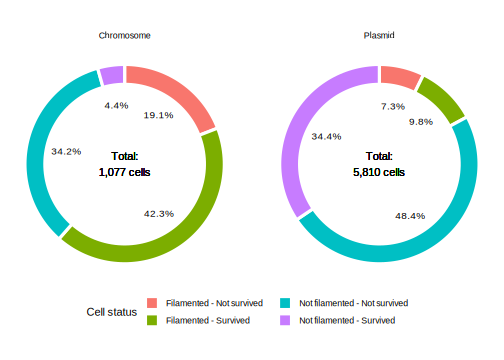
\includegraphics[width=1\linewidth]{02-experiment-analysis_files/figure-latex/experiment-03-cell-distribution-across-experiments-1} \caption[Cell classification and its distribution across experiments.]{\textbf{Cell classification and its distribution across experiments.} We define a \emph{filamented cell} as a cell whose length exceeded two standard deviations from the mean at any time during the experiment. A \emph{surviving cell} is a cell that was observed before and after exposure to the antibiotic. Accordingly, we removed from the analysis those cells that died before or were born after the exposure of the experiment. Therefore, we delimited the effect caused by the exposure to the antibiotic.}\label{fig:experiment-03-cell-distribution-across-experiments}
\end{figure}

\hypertarget{results}{%
\section{Results}\label{results}}

\hypertarget{length-gfp-crucial}{%
\subsection{Cell length and the amount of GFP are crucial in determining cell survival}\label{length-gfp-crucial}}

We evaluated the DsRed, GFP, and length values for each cell at
different time points: initial, filamentation, and end. This
preprocessing allowed us to observe and quantify each cell at critical
times in the experiment and eliminate noise or signals outside the scope
of this investigation.

We define the \emph{initial time} as the first time we observed the cell in
the experiment. \emph{Filamentation time} equals when a cell reaches the
filamentation threshold (see Figure
\ref{fig:experiment-03-length-temporal-distribution}) for the first
time. We defined the \emph{end time} as the time of the last observation of
the cell. We decided to bound the end time for surviving cells to one
frame (10 min) after the end of antibiotic exposure so that the observed
signal would reflect the final stress responses.

When we compared the distributions of DsRed, GFP, and length for both
experiments, we observed its changes in its role for cell survival. In
Figure \ref{fig:experiment-03-dsred-temporal-distribution}, we show
that indistinctly and, as expected, surviving cells managed to eliminate
the antibiotic by the end time. In contrast, dead cells presented higher
levels of antibiotics (measured by proxy through the mean DsRed
intensity of the cell).





\begin{figure}
\includegraphics[width=1\linewidth]{02-experiment-analysis_files/figure-latex/experiment-03-dsred-temporal-distribution-1} \caption[DsRed temporal distribution.]{\textbf{DsRed temporal distribution.} To evaluate the incident effect of the antibiotic marked by DsRed on cells by class, we show its values at three key moments: start, filamentation (SOS), and end. The upper asterisks represent the significance value when comparing a group X to the filamented and surviving cell reference. Asterisks in a line indicate whether or not there is a significant difference in the survival of non-filamented cells. The black dots represent the mean of each group, and the lines that join them are a comparative guide. The extent of the black bars represents the distribution of the data. Although, at the initial time, we observe multiple significant differences, this is likely due to the intrinsic noise of the system since, as expected, the values are close to zero. We observed a difference between the surviving and non-filamented cells for the chromosomal strain for the SOS time, but the same did not occur for the plasmid strain. The final amount of DsRed makes a clear difference between survival and death.}\label{fig:experiment-03-dsred-temporal-distribution}
\end{figure}

On the other hand, GFP observations in Figure
\ref{fig:experiment-03-gfp-temporal-distribution} showed us two
essential things for cell classification: 1) The chromosomal strain did
not exhibit noticeable changes in GFP levels, and 2) filamented cells
were those that had low fluorescent intensities (low plasmid
copy-number) at the beginning of the experiment. For the final
observation times, GFP measurements indicated that among the cells that
did not filament, the ones that survived exhibited a reduced GFP
expression concerning cells killed by the antibiotic. Meanwhile, for the
filamented cells, whether surviving or dead, their GFP measurements
indicated no difference at the beginning or the end of the experiment,
suggesting the presence of other determinants of cell survival.





\begin{figure}
\includegraphics[width=1\linewidth]{02-experiment-analysis_files/figure-latex/experiment-03-gfp-temporal-distribution-1} \caption[GFP temporal distribution.]{\textbf{GFP temporal distribution.} To evaluate the incident effect of the GFP on cells by class, we used the same notation as in Figure \ref{fig:experiment-03-dsred-temporal-distribution}. The chromosomal strain exhibits variability in GFP at different time points, mainly due to experimental noise resulting from low fluorescent intensity values. As expected, in the plasmid strain, filamented cells had a lower initial GFP. At the time of filamentation, there appear to be differences in fluorescence between surviving and dead cells. However, in the end time, we observed that the surviving non-filamented cells have lower GFP values than the non-filamented dead cells and alive filamented cells.}\label{fig:experiment-03-gfp-temporal-distribution}
\end{figure}

Cell length was one of the factors that GFP expression levels could not
explain for cell survival. In Figure
\ref{fig:experiment-03-length-temporal-distribution}, we show that the
conclusions regarding filamentation were applicable for both chromosomal
or plasmid strains. For the initial times, filamented and survived cells
were shorter in length than those that died but longer than not
filamented cells of both classes, while non-filamented cells did not
differ from each other. We observed no length differences between cells
at filamentation time. Thus, survival could depend on other factors,
such as growth rate. At the final time, the results were well-defined.
Surviving cells had a greater length relative to their non-surviving
pair (\emph{i.e.}, dead filamented and non-filamented cells). However, for
filamented cells, surviving cells represent a distribution of higher
final length values in general but not as extensive as their dead
counterpart. Which we could explain as a length limit to which cells can
grow without dying. Nevertheless, we had no information to evaluate such
a hypothesis.





\begin{figure}
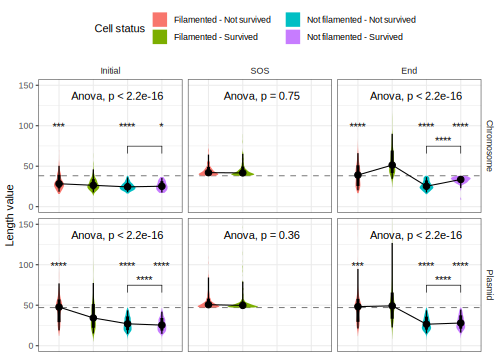
\includegraphics[width=1\linewidth]{02-experiment-analysis_files/figure-latex/experiment-03-length-temporal-distribution-1} \caption[Length temporal distribution.]{\textbf{Length temporal distribution.} To evaluate the incident effect of length on cells by class, we use the same notation as in Figure \ref{fig:experiment-03-dsred-temporal-distribution}. The observations for both strains, chromosomal or plasmid, are the same. In the beginning, the surviving filamented cells already have a difference in length concerning the rest of the classes. At the time of filamentation, there is no difference to help determine whether the cell will survive or not. Finally, in the final time, it seems that the surviving filamented cells have a greater length than the rest of the groups. However, this length is moderate compared to the excess length shown by non-surviving filamented cells. On the other hand, we highlighted the growth of the surviving non-filamented cells. Therefore, although they did not reach a length for us to classify as filamented, the cells did resort to filamentation.}\label{fig:experiment-03-length-temporal-distribution}
\end{figure}

Once we observed the effects of GFP expression levels and lengths in
determining whether a cell lives or dies, we projected the cells onto
the plane and painted them with their class status (See Figure
\ref{fig:experiment-03-cell-distribution-across-experiments}) to
determine whether these two variables contained the necessary
information to cluster the data correctly. In Figure
\ref{fig:experiment-03-just-initial-values}, we show the initial GFP
and length values projection. While, with some work, we could
contextually place the results in Figures
\ref{fig:experiment-03-gfp-temporal-distribution} and
\ref{fig:experiment-03-length-temporal-distribution}, the initial
values did not appear to determine the classes. Therefore, we explored
the final versus initial values differences in Figure
\ref{fig:experiment-03-metric-differences}. With this new
representation of the cells in the plane, we contextualized the
statistical results presented in Figures
\ref{fig:experiment-03-gfp-temporal-distribution} and
\ref{fig:experiment-03-length-temporal-distribution}. Besides, it
showed us that differences in length (\emph{i.e.}, filamentation) and
reductions in GFP expression are essential in determining cell survival.
Though, the clustering of cells by state is not completely separated,
which means that other variables are affection the experimental results
in cell survival.





\begin{figure}
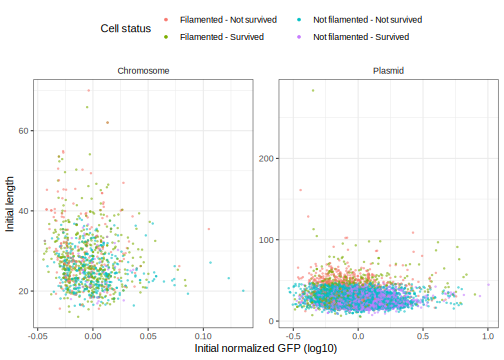
\includegraphics[width=1\linewidth]{02-experiment-analysis_files/figure-latex/experiment-03-just-initial-values-1} \caption[Experiment initial values.]{\textbf{Experiment initial values.} By positioning a cell in space based on its initial length and GFP values, we can see that class separation occurs, but not as a strong signal. Therefore, we concluded that although the initial state influences the result, this is not everything. For this, we have the example of the length changes throughout the experiment caused by filamentation. In this graph, the GFP scale is at log10 to help us observe those minor differences between the experiments.}\label{fig:experiment-03-just-initial-values}
\end{figure}





\begin{figure}
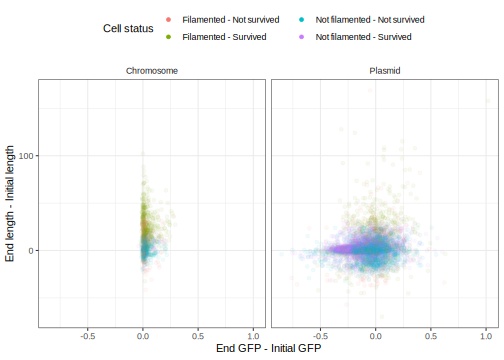
\includegraphics[width=1\linewidth]{02-experiment-analysis_files/figure-latex/experiment-03-metric-differences-1} \caption[Experiment initial values differences.]{\textbf{Experiment initial values differences.} By comparing the metric differences of the last observation and the first observation of a cell, we can separate mainly the surviving filamented cells from those that did not do it in both experiments (green dots). Meanwhile, cells with plasmids form a small accumulation of surviving cells that did not produce filament (purple dots). However, this has made a breakthrough in understanding what is affecting cell survival. There are still variables that we can include to understand this phenomenon better.}\label{fig:experiment-03-metric-differences}
\end{figure}

\hypertarget{number-of-divisions-and-cell-age-do-not-appear-to-play-a-clear-role-in-determining-cell-survival}{%
\subsection{Number of divisions and cell age do not appear to play a clear role in determining cell survival}\label{number-of-divisions-and-cell-age-do-not-appear-to-play-a-clear-role-in-determining-cell-survival}}

In Section \ref{length-gfp-crucial}, we explored how GFP variability
and cell length influence cell survival. However, Figures
\ref{fig:experiment-03-just-initial-values} and
\ref{fig:experiment-03-metric-differences} showed us the possibility of
other factors relevant to the phenomenon under study. As some papers in
the literature suggest, some of these other factors may be cell division
and chronological age (\emph{i.e.}, how much time has passed since the last
cell division at the time of exposure to a toxic agent)
\citep{moger-reischer2019, roostalu2008, heinrich2015}. Therefore, we chose
to observe these two metrics in experiments at a purely qualitative
level, i.e., without the inclusion of, e.g., metrics of membrane or cell
cycle properties \citep{Joseleau-Petit1999}.

Although we expected to see a small contribution, either by the number
of divisions or cell age, in Figures
\ref{fig:experiment-03-number-divisions} and
\ref{fig:experiment-03-time-since-last-division}, we could not observe
a precise effect of these variables on cell survival. Patterns that,
although they could have an explanation or biological significance, we
decided to omit as relevant in the characterization of our cells, since
the signal was not clear. However, we derived from this analysis a
slightly simpler variable that tells us whether a cell underwent a cell
division event or not. So it gives us a more generalized picture of the
contribution of division to cell survival (see Figure
\ref{fig:experiment-03-plasmid-pca-variable-contribution}).





\begin{figure}
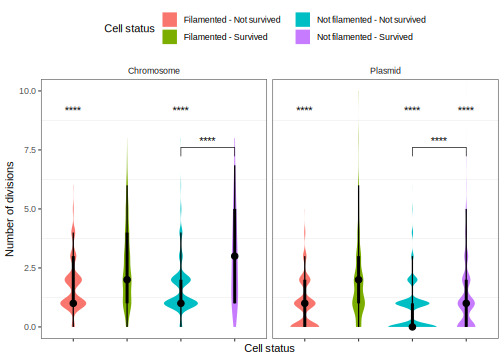
\includegraphics[width=1\linewidth]{02-experiment-analysis_files/figure-latex/experiment-03-number-divisions-1} \caption[Cell's number of divisions.]{\textbf{Cell's number of divisions.} Chromosomal cells exhibited more divisions for surviving classes and non-surviving filamented cells (\emph{i.e.}, purple, green, and red dots) relative to unchanged behavior in plasmid cells. Therefore, its contribution to filamentation remains uncertain.}\label{fig:experiment-03-number-divisions}
\end{figure}





\begin{figure}
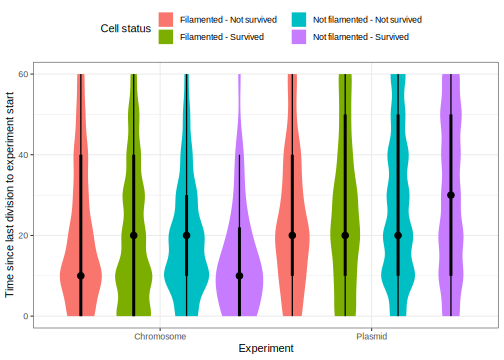
\includegraphics[width=1\linewidth]{02-experiment-analysis_files/figure-latex/experiment-03-time-since-last-division-1} \caption[Time elapsed since the last division at the beginning of the experiment.]{\textbf{Time elapsed since the last division at the beginning of the experiment.} The mean time of the last division before starting the experiment indicates that it did not influence the final result for chromosomal cells. There is a slight difference between the filamented-not survived cells and the rest for cells with plasmids. However, the signal does not appear to be strong on the survival role. Therefore, we conclude that we have no evidence to support that the time of the last division at the beginning of the experiment influences the final classification results.}\label{fig:experiment-03-time-since-last-division}
\end{figure}

\hypertarget{time-to-reach-filamentation-matters-in-determining-cell-survival}{%
\subsection{Time to reach filamentation matters in determining cell survival}\label{time-to-reach-filamentation-matters-in-determining-cell-survival}}

In Figures \ref{fig:experiment-03-dsred-temporal-distribution},
\ref{fig:experiment-03-gfp-temporal-distribution}, and
\ref{fig:experiment-03-length-temporal-distribution}, we showed how, at
the time of filamentation, DsRed and GFP levels appeared indifferent to
the cells. Therefore, we hypothesized that a possible variable that
could determine cell survival could be its time to activate its
anti-stress response system that causes filamentation. Furthermore, we
also guided our hypothesis by previous reports showing us how the gene
expression level can induce filamentation with tight temporal
coordination {[}x{]}.

While, for our analyses, we did not measure the concentration of
antibiotic that triggers filamentation per se, we indirectly quantified
its effect by using the time it took for a cell to reach a length at
which it is already considered a filamentating cell. Furthermore, to
recognize that the observed effect was a product of the experiment, we
decided to keep only filamented cells just once antibiotic exposure
began.

Figure \ref{fig:experiment-03-time-to-filamentation-filtered} shows how
filamentation times are narrower for chromosomal cells than for
plasmid-bearing cells. Then, we hypothesize that the effect could come
from the heterogeneity in the plasmid copy number in the population.
Also, interestingly, we observed that, for both experiments, cells that
survived had longer filamentation times than the cells that died. These
differences in response times suggest the following: 1) if the cell
grows too fast, it will reach a limit and start to accumulate
antibiotics constantly, and 2) if the cell grows too fast, it is likely
that the cost of maintaining an ample length for prolonged periods of
exposure will become counterproductive.





\begin{figure}
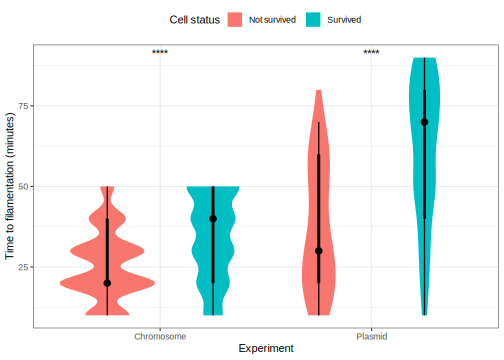
\includegraphics[width=1\linewidth]{02-experiment-analysis_files/figure-latex/experiment-03-time-to-filamentation-filtered-1} \caption[Time to filamentation filtered.]{\textbf{Time to filamentation filtered.} To quantify the effect of filamented to survive, we filtered those cells that filamented during the experiment. In this way, we normalize the start times for the calculation of the filamentation time. For both strains, the filamentation time had a more significant delay in the surviving cells.}\label{fig:experiment-03-time-to-filamentation-filtered}
\end{figure}

In Figure \ref{fig:experiment-03-initial-values-with-time}, we decided
to project the results of Figure
\ref{fig:experiment-03-time-to-filamentation-filtered} in a space
similar to the one described in Figure
\ref{fig:experiment-03-just-initial-values}. Thus, we separated our
data into cells that survived and cells that did not, and painted them
when it took them to reach their filamented state. We realized that,
indeed, by adding this temporal component to the initial variables of
length and GFP, we could separate surviving cells from dead cells to a
greater degree. However, it may still not be enough, and there are still
many other variables that play a crucial role in understanding the
ecology of stress and how some cells will be survivors or not.





\begin{figure}
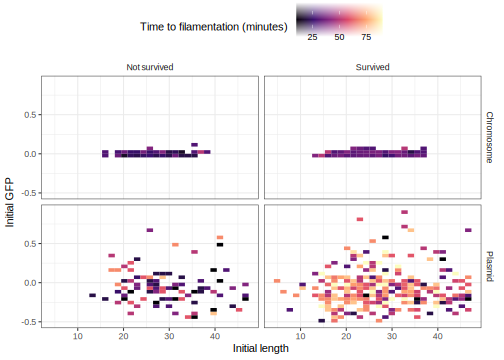
\includegraphics[width=1\linewidth]{02-experiment-analysis_files/figure-latex/experiment-03-initial-values-with-time-1} \caption[Experiment initial values with time to filamentation.]{\textbf{Experiment initial values with time to filamentation.} As in Figure \ref{fig:experiment-03-just-initial-values}, including the time it will take for cells to filament allows us to understand the phenomenon of survival better. Cells that filamented and survived generally have a much higher delay than their non-filamented peers for both strains (see Figure \ref{fig:experiment-03-time-to-filamentation-filtered}).}\label{fig:experiment-03-initial-values-with-time}
\end{figure}

\hypertarget{increasing-the-complexity-of-the-system-and-analyzing-it-in-an-unsupervised-way-allows-a-correct-classification-of-cell-states}{%
\subsection{Increasing the complexity of the system and analyzing it in an unsupervised way allows a correct classification of cell states}\label{increasing-the-complexity-of-the-system-and-analyzing-it-in-an-unsupervised-way-allows-a-correct-classification-of-cell-states}}

In the experiments, we observed the importance of GFP filamentation and
variability for cell survival. Similarly, we realized that other
variables must be affecting the final results. Filamentation and GFP
variability alone did not fully recapitulate the expected behavior of
the data. That is, the target variables did not capture the
heterogeneity of the system.

The inability to reproduce cell classification led us to question two
things: 1) the possibility that our sorting was wrong beforehand and 2)
we did not have enough variables to capture the study phenomenon. We
decided to take the unsupervised learning way to answer these subjects
because it allows us to project our data without a \emph{priori} knowledge
{[}x{]}.

We opted for the path of dimensionality reduction techniques where each
variable or feature is equivalent to one dimension. The essence of
dimensionality reduction is that it is not feasible to analyze each
dimension with many dimensions. Furthermore, dimensionality reduction
helps us counteract several problems such as reducing the complexity of
a model, reducing the possibility of overfitting a model, removing all
correlated variables, and, of course, visualizing our data in a two- or
three-dimensional space for better appreciation {[}x{]}. Improved
visualization and identification of essential variables are the main
reasons to guide and complement our research with this technique.

\hypertarget{principal-component-analysis-pca-emphasizes-the-importance-of-cell-length-and-its-gfp-in-cell-survival}{%
\subsubsection{Principal Component Analysis (PCA) emphasizes the importance of cell length and its GFP in cell survival}\label{principal-component-analysis-pca-emphasizes-the-importance-of-cell-length-and-its-gfp-in-cell-survival}}

The first dimensionality reduction technique we decided to use was
Principal Component Analysis (PCA) \citep{pearson1901, hotelling1936}.
Scientist mainly uses PCA to create predictive models or in Exploratory
Data Analysis (EDA). In our case, we only use it as an EDA.

For chromosomal and plasmid strain, in Figures
\ref{fig:experiment-03-chromosome-pca-new-coordinates} and
\ref{fig:experiment-03-plasmid-pca-new-coordinates}, we show the
projection of the first two principal components (PCs), respectively.
Figure \ref{fig:experiment-03-chromosome-pca-new-coordinates} separates
the manually annotated classes, surviving cells separated from
non-surviving cells. However, for Figure
\ref{fig:experiment-03-plasmid-pca-new-coordinates}, the class
separation was a bit rougher but allowed us to separate the surviving
filament cells from the dead ones.





\begin{figure}
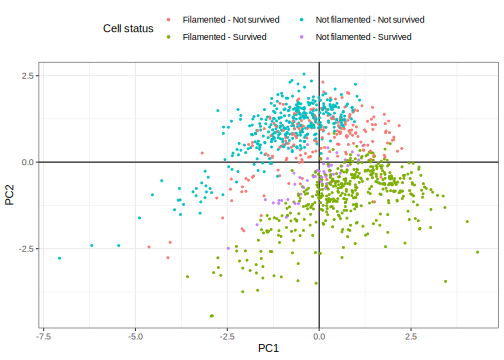
\includegraphics[width=1\linewidth]{02-experiment-analysis_files/figure-latex/experiment-03-chromosome-pca-new-coordinates-1} \caption[Principal Component Analysis of chromosomal strain.]{\textbf{Principal Component Analysis of chromosomal strain.} When integrating the information of different variables in a dimensionality reduction analysis, we observed a clear separation between the surviving cells and those that did not. The contributions that determined this phenomenon come mainly from the last amount of DsRed, GFP, and cell length (see Figure \ref{fig:experiment-03-chromosome-pca-variable-contribution}). Although it seems obvious, it effectively confirms that the temporal classification that we carry out makes sense. Longer length represents a greater uptake of antibiotics but in a much larger volume, so the net effect is an internal reduction of antibiotics (see Figure \ref{fig:model-01-cell-dimensions-relationship}).}\label{fig:experiment-03-chromosome-pca-new-coordinates}
\end{figure}





\begin{figure}
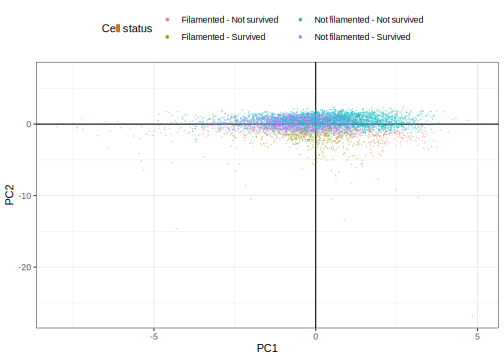
\includegraphics[width=1\linewidth]{02-experiment-analysis_files/figure-latex/experiment-03-plasmid-pca-new-coordinates-1} \caption[Principal Component Analysis of plasmid strain.]{\textbf{Principal Component Analysis of plasmid strain.} By integrating the information from different variables in a dimensionality reduction analysis, we observed a clear separation between the filamented and non-filamented cells. Said class separation is given by component 2 (Y-axis), which is determined primarily by the initial and final lengths of the cells (see Figure \ref{fig:experiment-03-plasmid-pca-variable-contribution}). Furthermore, the classification also allows us to separate those filamented cells that died from those that survived. Therefore, despite the increase in the system's complexity, length plays a role in determining survival.}\label{fig:experiment-03-plasmid-pca-new-coordinates}
\end{figure}

For their part, in Figures
\ref{fig:experiment-03-chromosome-pca-variable-contribution} and
\ref{fig:experiment-03-plasmid-pca-variable-contribution}, we show the
total contribution of each variable per PC for the chromosomal and
plasmid strain, respectively. Finding that, indeed, filamentation plays
a crucial role in determining cell survival. For example, for PC2, we
appreciated how the variable end DsRed directed the dots to the
positive side, while the variable end and start length directed the dots
to the opposing side. Therefore, we can support that filamentation has a
role in moving cells away from having higher amounts of DsRed.





\begin{figure}
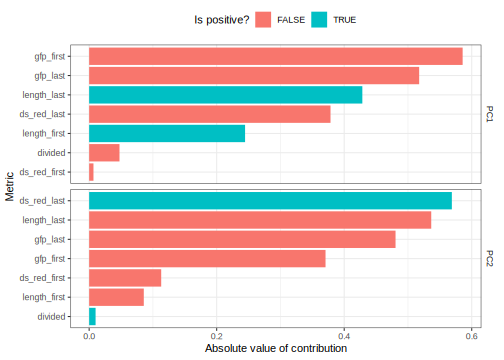
\includegraphics[width=1\linewidth]{02-experiment-analysis_files/figure-latex/experiment-03-chromosome-pca-variable-contribution-1} \caption[Variables contribution of Principal Component Analysis of chromosomal strain.]{\textbf{Variables contribution of Principal Component Analysis of chromosomal strain.} In the figure \ref{fig:experiment-03-chromosome-pca-new-coordinates}, we see that the classes we created manually reflected what we observed when performing a reduction of dimensions analysis. Here we show the individual contribution of each variable for the first two components. The variables that most affected components 1 and 2 (X-axis and Y-axis, respectively) are the final measurements of DsRed, GFP, length, and the initial amount of GFP. Given that they are chromosomal strains, we should note that this variability could be produced by intrinsic experimental noise that we could not remove. With that in mind, having the DsRed and the final length highlights the inherent role of cells by having increased its size.}\label{fig:experiment-03-chromosome-pca-variable-contribution}
\end{figure}





\begin{figure}
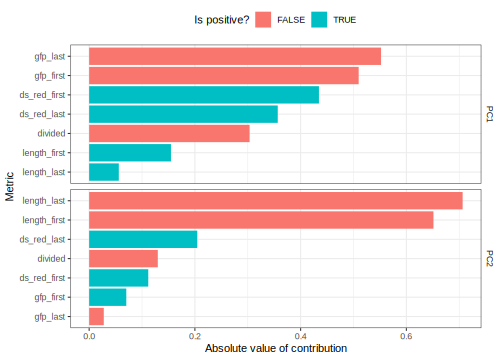
\includegraphics[width=1\linewidth]{02-experiment-analysis_files/figure-latex/experiment-03-plasmid-pca-variable-contribution-1} \caption[Variables contribution of Principal Component Analysis of plasmid strain.]{\textbf{Variables contribution of Principal Component Analysis of plasmid strain.} In Figure \ref{fig:experiment-03-plasmid-pca-new-coordinates}, we saw that we could separate the filamented cells from the non-filamented ones. The reduction analysis also shows a slight difference between surviving and dead cells within the small group of filamented cells. Here we offer the individual contribution of each variable for the first two components. For the first component (x-axis in Figure \ref{fig:experiment-03-chromosome-pca-new-coordinates}), the initial and final GFP measurements received mainly the variability. We expected this component's importance since, being a chromosomal strain, we hope that its inherent variation will be inherited into the system. On the other hand, the second component (Y-axis in Figure \ref{fig:experiment-03-chromosome-pca-new-coordinates}) was determined by the length of the cell. Factors that, in the chromosomal strain (see Figure \ref{fig:experiment-03-chromosome-pca-variable-contribution}), determined with the help of DsRed the separation between surviving and dead cells.}\label{fig:experiment-03-plasmid-pca-variable-contribution}
\end{figure}

\hypertarget{uniform-manifold-approximation-and-projection-umap-correctly-represents-the-local-structure-of-cell-states}{%
\subsubsection{Uniform Manifold Approximation and Projection (UMAP) correctly represents the local structure of cell states}\label{uniform-manifold-approximation-and-projection-umap-correctly-represents-the-local-structure-of-cell-states}}

Staying with only a one-dimensionality reduction technique was not an
option, so we used the UMAP technique \citep{mcinnes2018umap}. We mainly
decided to use UMAP for clustering purposes and see if the annotated
clusters corresponded to the manually annotated ones. UMAP has certain
advantages for these purposes, e.g., it preserves the global structure
across the whole space, so the distances between clusters matter.

In Figures \ref{fig:experiment-03-chromosome-umap-new-coordinates} and
\ref{fig:experiment-03-plasmid-umap-new-coordinates}, we show how,
using the same variables used in the ``PCA'' section, UMAP was able to
cluster the four proposed classes correctly. Interestingly, in Figure
\ref{fig:experiment-03-chromosome-umap-new-coordinates}, UMAP formed
three general groups and four for Figure
\ref{fig:experiment-03-plasmid-umap-new-coordinates}. However, in
general, UMAP clustered the surviving cells from those that did not
survived. On investigating why this separation occurred, we found that
the large groups coalesced into one another if we eliminated the
division variable. So, in a way, the division also has a role in
determining survival, but it is not essential or at least not
over-represented in our data.





\begin{figure}
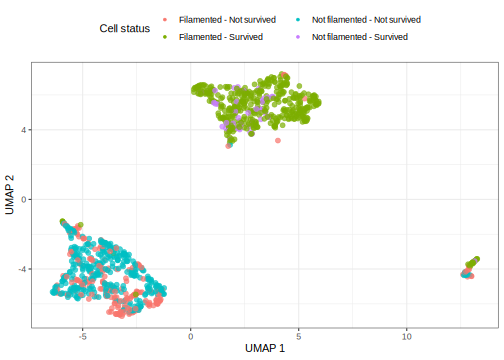
\includegraphics[width=1\linewidth]{02-experiment-analysis_files/figure-latex/experiment-03-chromosome-umap-new-coordinates-1} \caption[UMAP coordinates of chromosome strain.]{\textbf{UMAP coordinates of chromosome strain.} We represented the cells in a low dimensional space. This new projection made it possible to group the cells that survived and those that did not. Therefore, as in PCA Figure \ref{fig:experiment-03-chromosome-pca-new-coordinates}, this technique supports the manual classification that we carry out.}\label{fig:experiment-03-chromosome-umap-new-coordinates}
\end{figure}





\begin{figure}
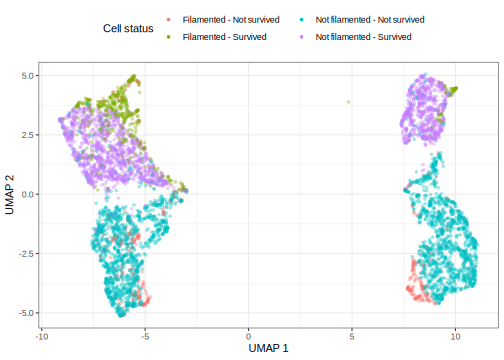
\includegraphics[width=1\linewidth]{02-experiment-analysis_files/figure-latex/experiment-03-plasmid-umap-new-coordinates-1} \caption[UMAP coordinates of plasmid strain.]{\textbf{UMAP coordinates of plasmid strain.} As in its \ref{fig:experiment-03-chromosome-umap-new-coordinates} pair, the representation in a low-dimensional space helped classify the cells, grouping mainly into four groups, two of survivors and two of non-survivors. The variable \emph{division} marks the separation of classes. The \emph{division} variable indicates whether a cell is divided during its lifetime or not. Together, the UMAP represents the manually assigned classes.}\label{fig:experiment-03-plasmid-umap-new-coordinates}
\end{figure}

\hypertarget{population-dynamics-reveal-how-filamentation-contributes-cell-survival}{%
\subsection{Population dynamics reveal how filamentation contributes cell survival}\label{population-dynamics-reveal-how-filamentation-contributes-cell-survival}}

From the full tracking dataset, we evaluated how the different cell
states behaved over time---for example, understanding how the cells
absorbed antibiotics or how they elongated in time. In contrast to the
dataset generated in the \ref{length-gfp-crucial} section, we did not
truncate the results 10 minutes after the antibiotic exposure. In this
way, we were able to observe cell behavior before and after the presence
of the toxic agent.

In Figure \ref{fig:experiment-04-status-with-dead}, we observed a small
fraction of cells that were already filamentous without exposure to the
toxic agent in both cell strains. However, after the onset of antibiotic
exposure at minute 60, we observed increases in the proportion of
filamented cells. It is interesting to note how filamented cells grew
after antibiotic exposure for the chromosomal strain. We speculate that
this post-antibiotic growth exists because, once the SOS system that
triggers filamentation is activated, the system continues to grow until
it reaches a limit regardless of whether the damaging agent is still
present or not \citep{justiceMorphologicalPlasticityBacterial2008, mückl2018}. Moreover, we observed how the cells start to divide again
after some time because the proportion of non-filament cells starts to
grow while the filament cells start to divide. We observed the same
effects for the plasmid strain. However, by experimental design, the
number of filament cells expected was much lower.





\begin{figure}
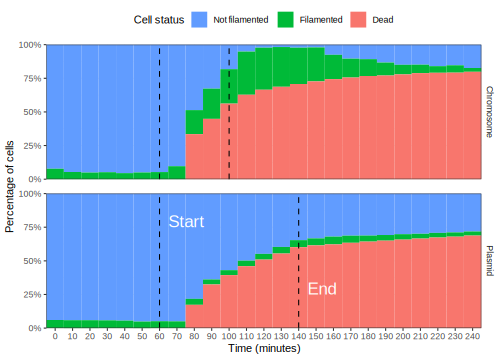
\includegraphics[width=1\linewidth]{02-experiment-analysis_files/figure-latex/experiment-04-status-with-dead-1} \caption[Population status over time.]{\textbf{Population status over time.} We calculate how many cells of each type existed for each time point: non-filamented and filamented living cells (blue and green areas, respectively) and dead cells (red area; we considered \emph{dead} cells as those cells that existed at one time and then stopped tracking). The black vertical lines represent the start and end of antibiotic exposure for each experiment. The effect of filamentation and its spread after exposure to the antibiotic is evident for the chromosomal strain. The experiment was finalized with the resolution of the cells when they returned to their non-filamented state. For its part, for the plasmid strain, it is observed how the filamented cells begin to appear slowly. Their proportion is as expected, given that the population had a wide distribution of GFP that allowed them to combat exposure to the antibiotic.}\label{fig:experiment-04-status-with-dead}
\end{figure}

In Figure \ref{fig:experiment-04-metrics-over-time}, we showed how once
antibiotics exposure began, those cells that died had a much faster
increase in DsRed than those that did manage to live, regardless of
whether they filamented or not. On the other hand, surviving cells
managed to maintain their DsRed levels relatively stable. We noted that
length was critical for the surviving cells for the chromosomal strain
by turning to the GFP and length variables for a temporal explanation.
Even cells categorized as non-filamented reached the filamentation
threshold minutes after antibiotic exposure. However, the distinction of
live or dead filamented cells was not as evident as expected. As for
cells with plasmids, the effect on GFP for surviving cells was
maintained for filamented cells and decreased for non-filamented cells.
For the filament cells that died, we showed that they had, on average, a
much longer initial length than the surviving cells, so we also consider
it as a necessary factor in understanding which variables affect cell
survival.





\begin{figure}
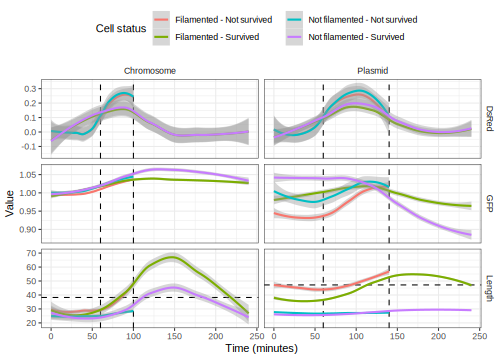
\includegraphics[width=1\linewidth]{02-experiment-analysis_files/figure-latex/experiment-04-metrics-over-time-1} \caption[Population measurements over time.]{\textbf{Population measurements over time.} The colored lines symbolize the average value of each metric at each instant of time, while its surrounded gray shaded area represents the 95\% confidence interval. The vertical lines represent the start and end of antibiotic exposure. The horizontal line in the length metric symbolizes the threshold to consider a cell filament. We observed a faster increase of DsRed for the non-surviving populations in both experiments. Regarding the GFP metric, the behavior is relatively stable for the chromosomal strain. In contrast, for the plasmid strain, a decline in GFP is observed for the population that did not survive. For the length metric, it is interesting to note how the chromosome cells that did not filament continued to grow past the filamentation threshold once the exposure to the antibiotic in the chromosomal strain had ended. On the other hand, the filamented and dead cells seem to have a greater length from the beginning for the plasmid strain.}\label{fig:experiment-04-metrics-over-time}
\end{figure}

\hypertarget{heterogeneity-in-plasmid-copy-number-allows-various-forms-of-survival-in-addition-to-filamentation}{%
\subsection{Heterogeneity in plasmid copy-number allows various forms of survival in addition to filamentation}\label{heterogeneity-in-plasmid-copy-number-allows-various-forms-of-survival-in-addition-to-filamentation}}

We are confident that filamentation has a fundamental role in
determining cell survival, with what we have shown so far. However, for
plasmid cells, we have a component that is of our complete interest;
heterogeneity. Each cell can possess a different plasmid copy-number;
thus, each could show a different behavior under stress
\citep{sanmillan2016}. For instance, heterogeneity can produce resistant
cells that do not suffer damage, susceptible cells, and cells that form
filaments to mitigate environmental stress.

To study the effect of variability in plasmid copy number in the
survival probability of the population, we decided to group cells by the
proportion of initial GFP with respect to the population maximum. We
defined 100\% of the population as the number of total cells at the onset
of antibiotic exposure. Figure
\ref{fig:experiment-04-proportion-living-cells-gfp-by-row} shows how
the cells with the highest amount of GFP remained unchanged once
antibiotic exposure began, while the rest of the cells started to
decrease their percentage of surviving cells. However, the decrease was
not linear. On the contrary, we observed a bi-modal distribution on the
reduction of live cells. An average GFP point provided higher survival
than a point below or above the average (except for cells very close to
the population maximum).





\begin{figure}
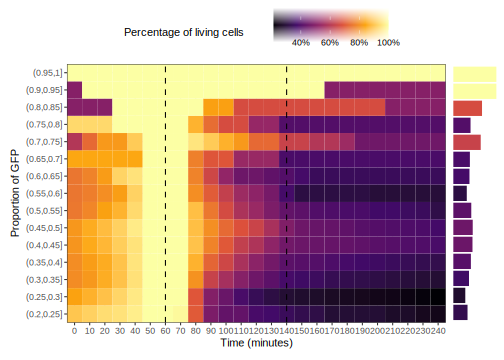
\includegraphics[width=1\linewidth]{02-experiment-analysis_files/figure-latex/experiment-04-proportion-living-cells-gfp-by-row-1} \caption[Population survivals binned by initial GFP over time.]{\textbf{Population survivals binned by initial GFP over time.} We categorized the cells' GFP into ranges of proportions 0.05 concerning the maximum amount of GFP in the population. 100\% cells per bin of GFP was taken as the number of cells one frame before the start of exposure to the antibiotic (minute 50). Therefore, dark to light colors represent a generation of new cells, and light to dark colors the death of cells. The black vertical bars represent the start and end of the antibiotic exposure. Bars size and color on the right represent the percentage of the living cells 10 minutes after the end of the experiment. As shown in Figure \ref{fig:experiment-04-gfp-survival-probability}, we showed that the surviving cells appear to follow something similar to a bimodal distribution. More cells survive with a moderate amount of GFP or with an amount close to the maximum of the population.}\label{fig:experiment-04-proportion-living-cells-gfp-by-row}
\end{figure}

Therefore, what we observed was a bimodal distribution for GFP-dependent
cell survival. In order to show this effect more clearly, in Figure
\ref{fig:experiment-04-gfp-survival-probability}, we plotted the
survival probability for each GFP bin without normalizing for the
population maximum. This new plot allowed us to observe how the bimodal
survival distribution occurs for cells that did not grow as filaments,
whereas cells that filament increase their survival probability
gradually as they have more initial GFP (see also Figure
\ref{fig:experiment-03-gfp-temporal-distribution}).





\begin{figure}
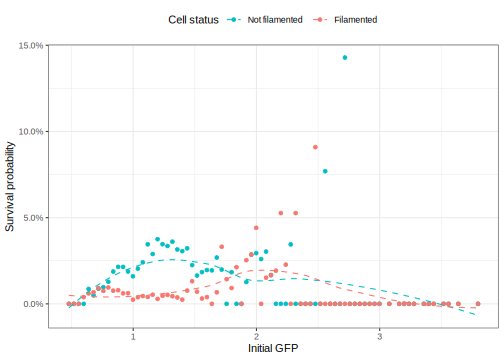
\includegraphics[width=1\linewidth]{02-experiment-analysis_files/figure-latex/experiment-04-gfp-survival-probability-1} \caption[Plasmid initial GFP survival probability.]{\textbf{Plasmid initial GFP survival probability.} We calculated the survival probability after comparing the population distributions of GFP with those of the cells that managed to survive. To assess survival by GFP, we only used plasmid cells. For non-filamented cells (blue dots), a bell forms with an upturned tail. On the other hand, for the filamented cells (red dots), a continuous increase in survival is shown just when it seems that the probability of the non-filamented cells has decreased. In global, much GFP has higher resistance, but an average GFP value without filamentation also increases the probability of survival.}\label{fig:experiment-04-gfp-survival-probability}
\end{figure}

As in Figure \ref{fig:experiment-04-gfp-survival-probability}, in
Figure \ref{fig:experiment-04-length-survival-probability}, we show the
survival probability given an initial length. We observe that survival
is higher for cells that did not grow as filament if the initial length
was less than the average. In contrast, for filamented cells, the
probability of survival increased as cells length was longer at the
beginning of the experiment (see also Figure
\ref{fig:experiment-03-length-temporal-distribution}). However, it is
noteworthy that the probability of survival had a limit in which a
higher initial length meant a lower probability of survival (see red
dotted lines in Figure
\ref{fig:experiment-04-length-survival-probability}).





\begin{figure}
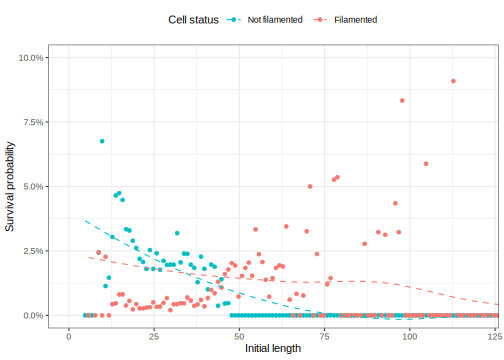
\includegraphics[width=1\linewidth]{02-experiment-analysis_files/figure-latex/experiment-04-length-survival-probability-1} \caption[Plasmid initial length survival probability.]{\textbf{Plasmid initial length survival probability.} We calculated the survival probability after comparing the population distributions of length with those of the cells that managed to survive. For non-filamented cells (blue dots), the survival probability is higher for those cells with initial lengths and small. It seems to decrease with a more extensive initial size. For their part, for filamented cells (red dots), the probability of survival increases according to their length but then declines when the cells are too long at first (see red dotted line). Therefore, in general, a small and moderate length or an initial length already filamented from the beginning increases the chances of survival.}\label{fig:experiment-04-length-survival-probability}
\end{figure}

\hypertarget{discussion}{%
\section{Discussion}\label{discussion}}

Here, we evaluated different variables that could determine cell
survival upon exposure to toxic agents by studying two experimental
populations of \emph{E. coli}, one strain with a resistance gene on the
chromosome and the other on multicopy plasmids. We identified two
variables that are predominantly responsible for cell survival: cell
length and GFP amount related to the cell's inherent resistance to the
toxic agent and heterogeneity in response times.

On the other hand, as other studies have already mentioned
\citep{heinrich2015, wang2009}, we examined cell activity and youth in a
minimalistic way. While the distribution of the number of divisions
exemplifies a broader and more uniform range for the surviving cells,
the cells that died showed a tendency to a lower number of divisions.
However, for the study of cellular youth at the time of exposure to the
toxic agent, the results did not show a clear pattern of behavior for
cell fate determination. Therefore, it would be interesting to study
cellular youth at a higher level of complexity in future studies to
understand its contribution to cell survival.

Interestingly, when we used temporal measurements of cell length, GFP,
DsRed, and if a cell divided, we could recapitulate, for the most part,
the fates of cellular states (see Sections \ref{length-gfp-crucial} and
\ref{increasing-the-complexity-of-the-system-and-analyzing-it-in-an-unsupervised-way-allows-a-correct-classification-of-cell-states}).
Thus, increasing the system's complexity led to better clustering cell
states, but not how these factors interact biologically in determining
cell survival. Therefore, we decided to postulate a mathematical model
that helps us understand the critical components in cell survival.

\hypertarget{model-analysis}{%
\chapter{Models to the rescue; filamentation abstraction}\label{model-analysis}}

\hypertarget{introduction-3}{%
\section{Introduction}\label{introduction-3}}

By integrating information from the environment, cells can alter their
cell cycle. For instance, some cells arrest the cell division in the
presence of toxic agents but continue to grow. Previous studies have
shown that this filamentation phenomenon provides a mechanism that
enables cells to cope with stress, which leads to an increase in the
probability of survival \citep{justiceMorphologicalPlasticityBacterial2008}.
For example, filamentation can be a process capable of subverting innate
defenses during urinary tract infection, facilitating the transition of
additional rounds of intracellular bacterial community formation
\citep{justiceFilamentationEscherichiaColi2006}.

Although filament growth can help mitigate environmental stress (e.g.,
by activating the SOS response system
\citep{justiceMorphologicalPlasticityBacterial2008}), the evolutionary
benefits of producing elongated cells that do not divide are unclear.
Here, we proposed a mathematical model based on ordinary differential
equations that explicitly considers the concentration of intracellular
toxin as a function of the cell's length (see Equation
\eqref{eq:model-equation}). The model is built based on the growth ratio
of measurements of the surface area (\(SA\)) and the cell volume (\(V\)),
whereby the uptake rate of the toxin depends on the \(SA\). However, \(V's\)
rate of change for \(SA\) is higher than \(SA\) for \(V\), which results in a
transient reduction in the intracellular toxin concentration (see Figure
\ref{fig:model-01-cell-dimensions-relationship}). Therefore, we
hypothesized that this geometric interpretation of filamentation
represents a biophysical defense line to increase the probability of a
bacterial population's survival in response to stressful environments.





\begin{figure}
\includegraphics[width=1\linewidth]{downloadFigs4latex_03-model-analysis/model-01-cell-dimensions-relationship} \caption[Cell dimensions relationship.]{\textbf{Cell dimensions relationship.} We evaluated the resulting geometric properties on a grid of side lengths and radii with a pill-shaped cell. We can see that by maintaining a constant radius (typical case in bacteria such as \emph{E. coli}) and increasing the side length, the surface area / volume relationship (\(SA/V\)) tends to decline since the \(V\) will grow at a higher rate than the \(SA\).}\label{fig:model-01-cell-dimensions-relationship}
\end{figure}

\hypertarget{filamentation-model}{%
\section{Filamentation model}\label{filamentation-model}}

Let us assume the shape of cells is a cylinder with hemispherical ends.
Based on this geometric structure, a nonlinear system of differential
equations governing filamentation can be written as follows:

\begin{equation}
\begin{split}
\frac{dT_{int}}{dt} &= T_{sa} \cdot (T_{ext}(t) - T_{vol}) - \alpha \cdot T_{ant} \cdot T_{int} \\
\frac{dL}{dt} &= 
  \begin{cases} 
    \beta \cdot L,& \text{if } T_{int} \geq T_{sos},  t \geq \tau_{sos} + \tau_{delay} \text{ and } L < L_{max}  \\
    0,            & \text{otherwise}
  \end{cases}
\end{split}
\label{eq:model-equation}
\end{equation}

It considers the internal toxin (\(T_{int}\)) and the cell length (\(L\)) as
variables. \(T_{sa}\) and \(T_{vol}\) represent the surface area and volume
of the toxin in the cell, respectively. \(T_{ext}(t)\) is a function that
returns the amount of toxin in the cell medium. \(T_{anti}\) and \(\alpha\)
symbolize the amount of antitoxin and its efficiency rate, respectively.
\(\beta\) as the rate of filamentation. \(L_{max}\) is the maximum size that
the cell can reach when filamentation is on. \(T_{sos}\) and \(T_{kill}\)
are thresholds for filamentation and death, respectively. Finally,
\(\tau_{delay}\) is the amount of time required to activate filamentation
after reaching the \(T_{sos}\) threshold.

\hypertarget{numerical-results}{%
\section{Numerical results}\label{numerical-results}}

\hypertarget{filamentation-provides-transient-resistance-to-stressful-conditions}{%
\subsection{Filamentation provides transient resistance to stressful conditions}\label{filamentation-provides-transient-resistance-to-stressful-conditions}}

When growing rod-shaped bacterial cells under constant conditions, the
distribution of lengths and radii is narrow
\citep{schaechterGrowthCellNuclear1962}. However, when growing under stress
conditions, some cells produce filaments
\citep{schaechterDependencyMediumTemperature1958}. This phenomenon may depend
on the SOS response system \citep{bosEmergenceAntibioticResistance2015},
which can repair DNA damage, giving the cell greater chances of
recovering and surviving under stress conditions. Besides, the SOS
response has been reported to have precise temporal coordination in
individual bacteria \citep{friedmanPreciseTemporalModulation2005}. Among the
stress conditions that can trigger the SOS response is exposure to
beta-lactam antibiotics \citep{millerSOSResponseInduction2004}.

In general, filamentation has been studied as an unavoidable consequence
of stress. However, we considered filamentation an active process that
produces the first line of defense against toxic agents. Therefore, a
differential equation model was proposed that assesses the change in the
amount of internal toxin as a function of cell length. At the core of
this model, we include the intrinsic relationship between the surface
area and the capsule volume since it is vital in determining cell size
\citep{harrisRelativeRatesSurface2016}.

In figure \ref{fig:model-01-filamentation-model-ramp-signal}, cells
grow in a ramp-shaped external toxin signal without considering a
toxin-antitoxin system.As time progresses, the toxin in the external
environment increases, so the cell raises its internal toxin levels. At
approximately time \(22\), any cell reaches \(T_{sos}\). The control cell
(unable to filament) and the average cell (capable of filamenting) reach
the death threshold, \(T_{kill}\), at times \(31\) and \(93\) (hatched and
solid black lines), respectively. Therefore, under this example, the
cell has increased its life span three times more than in control by
growing as a filament (green shaded area versus orange shaded area). In
turn, figure \ref{fig:model-01-filamentation-model-ramp-signal} also
shows stochastic simulations of the system in the intake of internal
toxins. Considering that cell growth and death processes are inherently
stochastic, stochastic simulations would be a better approximation.
However, from now on, we will continue with the study of the
deterministic model.





\begin{figure}
\includegraphics[width=1\linewidth]{downloadFigs4latex_03-model-analysis/model-01-filamentation-model-ramp-signal} \caption[Effect of filamentation on intracellular toxin concentration.]{\textbf{Effect of filamentation on intracellular toxin concentration.} In the presence of an extracellular toxic agent, the intracellular concentration of the toxin (\(T_{int}\)) increases until reaching a damage threshold that triggers filamentation (\(T_{sos}\), blue point), increasing cell length (\(L\)). When filamentation is on, the cell decreases \(T_{int}\) due to the intrinsic relationship between surface area and cell volume. When the cell reaches its maximum length, it eventually dies if the stressful stimulus is not removed (\(T_{kill}\), red dot). The hatched line represents a cell that can not grow as filament. The orange shaded area is the time between stress and the non-filament cell's death, while the green shaded area represents the temporal gain for doing so. The blue background lines represent stochastic simulations of the same system.}\label{fig:model-01-filamentation-model-ramp-signal}
\end{figure}

\hypertarget{filamentation-increases-the-minimum-inhibitory-concentration}{%
\subsection{Filamentation increases the minimum inhibitory concentration}\label{filamentation-increases-the-minimum-inhibitory-concentration}}

In other to characterize the degree of resistance, dose-response
experiments determine the Minimum Inhibitory Concentration (MIC)
\citep{andrews2001, andrewsDeterminationMinimumInhibitory2002}. Bacteria are
capable of modifying their MIC through various mechanisms, for example,
mutations \citep{lambertBacterialResistanceAntibiotics2005}, impaired
membrane permeability \citep{satoOuterMembranePermeability1991}, flux pumps
\citep{webberImportanceEffluxPumps2003}, toxin-inactivating enzymes
\citep{wrightBacterialResistanceAntibiotics2005}, and plasticity phenotypic
\citep{justiceMorphologicalPlasticityBacterial2008}. The latter is our
phenomenon of interest because it considers the change in shape and
size, allowing us to study it as a strategy to promote bacterial
survival.

We decided to analyze the MIC change caused by filamentation through
stable exposure experiments of different toxin amounts at other exposure
times. Computational simulations show that when comparing cells unable
to filament with those that can, there is an increase in the capacity to
tolerate more generous amounts of toxin, increasing their MIC (see
Figure \ref{fig:model-02-toxin-exposure-experiment}). Therefore, it
confers a gradual increase in resistance beyond filamentation's role in
improving the cell's life span as the exposure time is longer.





\begin{figure}
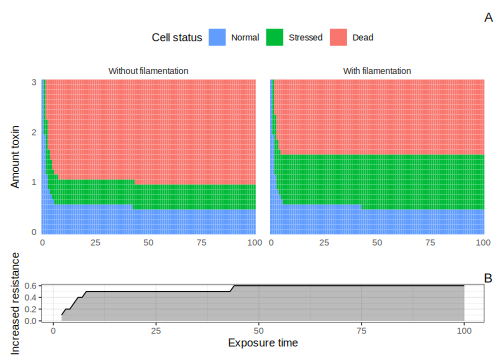
\includegraphics[width=1\linewidth]{03-model-analysis_files/figure-latex/model-02-toxin-exposure-experiment-1} \caption[Effect of filamentation on minimum inhibitory concentration (MIC).]{\textbf{Effect of filamentation on minimum inhibitory concentration (MIC).} By exposing a cell to different toxin concentrations with stable signals, the cell achieves a set MIC for conditions without or with filamentation (separation between stressed and dead state) for each exposure time, without representing a change for the normal state cells' points (blue zone). Thus, the green line represents a gradual MIC increase when comparing each MIC between conditions for each exposure time.}\label{fig:model-02-toxin-exposure-experiment}
\end{figure}

\hypertarget{heterogeneity-in-the-toxin-antitoxin-system-represents-a-double-edged-sword-in-survival-probability}{%
\subsection{Heterogeneity in the toxin-antitoxin system represents a double-edged sword in survival probability}\label{heterogeneity-in-the-toxin-antitoxin-system-represents-a-double-edged-sword-in-survival-probability}}

One of the SOS response system properties is that it presents
synchronous activation times within homogeneous populations
\citep{friedmanPreciseTemporalModulation2005}. It has constant gene
expression rates that help it cope with stress; however, it is possible
to introduce variability by considering having multicopy resistance
plasmids \citep{million-weaverMechanismsPlasmidSegregation2014}. Therefore,
the response times would have an asynchronous behavior at the global
level but synchronous at the local level.

To include this observation into the model, we include a negative term
to the internal toxin representing a toxin-antitoxin system. Therefore,
the model now has an efficiency rate of the antitoxin and a stable
amount per cell. We simulate the effect of the toxin-antitoxin system
variation within a \(1000\)-cell population; we initialize each one with
similar initial conditions, except for the amount of internal antitoxin,
defined as \(T_{anti} \sim N(\mu, \sigma)\). Considering that \(T_{anti}\)
values \(< 0\) are equal to \(0\). For each experiment, \(\mu = 25\), while it
was evaluated in the range \([0-20]\). For the generation of pseudo-random
numbers and to ensure the results' reproducibility, the number \(42\) was
considered seed.

As shown in Figure \ref{fig:model-02-antitoxin-experiment}, when we
compare heterogeneous populations in their toxin-antitoxin system, we
can achieve different population dynamics, that is, changes in the final
proportions of cell states; normal, stressed, and dead. This difference
is because the cell sometimes has more or less antitoxin to handle the
incoming stress situation.





\begin{figure}
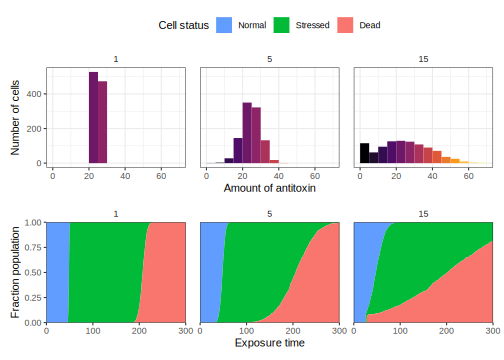
\includegraphics[width=1\linewidth]{03-model-analysis_files/figure-latex/model-02-antitoxin-experiment-1} \caption[Variability in the toxin-antitoxin system produces different proportions of cell states.]{\textbf{Variability in the toxin-antitoxin system produces different proportions of cell states.} Histograms represent the distribution of antitoxin quantity, while the curves represent the population's fraction over time. The cell will start to filament after reaching a certain internal toxin threshold, \(T_{sos}\). Therefore, the expected global effect on the population's response times based on the amount of antitoxin is asynchronous, while at the local level, it is synchronous. Consequently, different proportions are presented in the cellular states since some cells will activate the filamentation system before and others later.}\label{fig:model-02-antitoxin-experiment}
\end{figure}

Considering that the toxin-antitoxin system's variability can modify the
proportions of final cell states, a question arose about heterogeneity
levels' global behavior. To answer this question, we evaluate the
probability of survival for each population, defined by its distribution
of antitoxin levels. In this way, we characterized the population
survival probability function into three essential points according to
its effect: negative, invariant, and positive (see Figure
\ref{fig:model-02-survival-probability}). Furthermore, these points are
relative to the homogeneous population's death time in question
(\(\tau_{kill}\)): when \(t < \tau_{kill}\) will represent a detrimental
effect on survival, \(t = \tau_{kill}\) will be independent of
variability, and \(t > \tau_{kill}\) will be a beneficial point for
survival. Therefore, we concluded that the effect of heterogeneity in a
toxin-antitoxin system represents a double-edged sword.





\begin{figure}
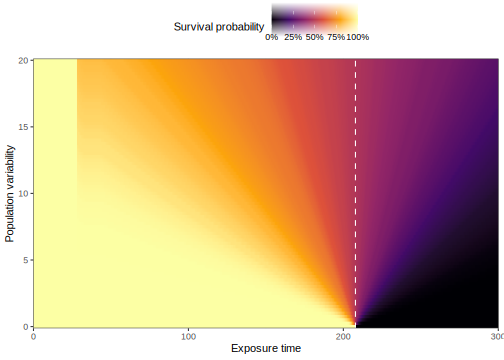
\includegraphics[width=1\linewidth]{03-model-analysis_files/figure-latex/model-02-survival-probability-1} \caption[Effect of variability on the toxin-antitoxin system.]{\textbf{Effect of variability on the toxin-antitoxin system.} The color of the heatmap is representative of the fraction of living cells at exposure time. The white vertical line represents the death time of the homogeneous population (\(\tau_{kill}\)). At \(t < \tau_{kill}\), it is shown that the fraction of survivors decreases as the variability in the population increases. When \(t = \tau_{kill}\), the variability does not affect the fraction of survivors, but it represents a percentage improvement for the homogeneous population. Finally, when \(t > \tau_{kill}\), the heterogeneity of the population favors survival.}\label{fig:model-02-survival-probability}
\end{figure}

\hypertarget{benefits-and-limitations-of-the-model}{%
\section{Benefits and limitations of the model}\label{benefits-and-limitations-of-the-model}}

Today, there have been advancements in the number of techniques that
have allowed it to extend quantitative analyses to individual cells'
dynamic observations \citep{camposConstantSizeExtension2014, meldrumFacultyOpinionsRecommendation2005, sliusarenkoHighthroughputSubpixelPrecision2011, taheri-araghiCellSizeControlHomeostasis2017, ursellRapidPreciseQuantification2017}. Therefore, studying their
cellular behavior every day from medium to medium can be somewhat
reproducible, facilitating the association of complex biological
functions in simple mathematical equations
\citep{neidhardtBacterialGrowthConstant1999}.

Here, we proposed a mathematical model showing that filamentation could
serve as a population's resilience mechanism to stress conditions.
Finding that filamentation's net effect generates an additional window
of time for the cell to survive, decreasing the toxin's intracellular
concentration. However, we also found that a side effect of
filamentation is to increase the cell's minimum inhibitory
concentration. On the other hand, when we introduce variability in the
amount of antitoxin in a cell population, we found that heterogeneity
can be a double-edged sword, sometimes detrimental and sometimes
beneficial, depending on the time of exposure to the toxic agent.

Due to the above, despite being simple, the model could have the ability
to recapitulate the behavior seen in nature from variables that we can
calculate easily with single-cell measurements. However, in other
situations, it could be helpful to consider the addition of variables
such as cell wall production and peptidoglycans' accumulation, among
others. Notwithstanding the lack of parameters that are a little closer
to reality, confirming that the model can work under experimental
conditions would represent an achievement due to its explanatory
simplicity, starting, in this way, the path of the study of
filamentation oriented to the ecology of stress.

\hypertarget{general-discussion}{%
\chapter{Discussion}\label{general-discussion}}

Bacterial cell survival is part of a complex biological system, which is
one of the fundamental problems of the health sector in this century. In
this work, we have analyzed the role of filamentation in cell survival
through multiple levels of complexity. Inquiring, one step at a time,
into the ecology of bacterial stress.

First, we exposed two bacterial strains, one with an antibiotic
resistance gene on the chromosome and one on multicopy plasmids, in a
stressful environment with ampicillin. In both cases, we observed four
states in the cells at the end of the experiment: live filamented, live
non-filamented, dead filamented, and dead non-filamented cells. By
inspecting the specific characteristics of each category, we were able
to identify that cell length was indeed related to the probability of
survival. In addition, we showed that each cell's inherent resistance
defined whether or not filamentation would occur for the plasmid strain,
where low resistance values were conducive to filamentation.

However, the growth rate was critical in determining the final cellular
state. We observed that moderate growths mainly were related to
survival. In contrast, rapid growth was associated with cell death.
Previous findings, in addition, could have other explanations that are
not mutually exclusive, such as the cell cycle or how fast a given cell
was dividing. So the contribution of these variables in conjunction with
filamentation could be a future study of interest to improve our
understanding of cell survival.

Our next step was to abstract the fundamental information to define a
mathematical model that would help us better understand the workings of
filamentation in cell survival. We postulated a mathematical model built
from a system of differential equations that considers the cell's
geometric relationships (i.e., a pill shape) against exposure to a toxic
substance in the environment. We assume that the consumption of
antibiotics by the cell is perceived through its surface area (\(SA\)),
while the cell volume (\(V\)) defines its concentration. Consequently,
since the rate of change of \(SA\) is lower than \(V\), this results in a
transient reduction in the intracellular concentration of the toxin.

In the experiments, we showed how cells begin to filament upon a pulse
of antibiotics, and from this, it would begin their bid for survival.
The model allowed us to consider thousands of different cells to
precisely determine the impact of filamentation on their survival. For
instance, upon incremental exposure to the toxic substance, a cell can
increase its lifetime window by simply growing. If the antibiotic wears
off before the cell reaches a threshold of death for some reason, it
will have paid off; the cell will have won the bet, and it will have
survived. Conversely, if a cell can not grow as a filament, it will
depend entirely on its inherent resistance levels.

In addition to the increase in the expected lifetime of the cell upon
exposure to a toxic agent, the model showed us that filamentation could
confer an increase in the Minimum Inhibitory Concentration (MIC). So if
a cell can grow as filament, a higher amount of the toxic agent will be
needed to kill it. However, bacteria generally live in heterogeneous
populations, and sometimes their inherent resistance levels will play a
vital role in their survival.

The model showed us that heterogeneity in toxin-antitoxin response
systems could represent a double-edged sword for cell survival depending
on the time of exposure to the toxin. Heterogeneity could be favorable
for survival if the time of exposure to the toxic agent is longer than
the time at which the population without heterogeneity dies completely,
while it would be detrimental otherwise. Thus, globally, filamentation,
both at the individual and population scale, is crucial for resilience.

However, although our model's advantages are its simplicity, ease of
interpretation, and reproducibility of the biological phenomenon in
question, it also entails limitations to be considered in further work.

Our model assumes zero growth if the cell does not reach the
filamentation threshold. While this may be true at the population
average level, the reality is that cells are constantly growing and
dividing. Integrating constant growth and division events could help us
understand in more detail how, under what conditions, and why
filamentation might be beneficial or detrimental when considering new
transition states.

Another limiting factor is the lack of a system that penalizes prolonged
filamentation. Once the cell filaments, our model considers only two
possible scenarios, the cell can either continue with filamentation for
its entire lifetime or die from crossing a toxic agent threshold.
However, we can suggest that maintaining a filamentary state carries an
energetic and membrane material cost that may be difficult to supply.
Thus, a cell could die from spending too long in the filamentation state
if exposure to the toxic agent does not cease.

The model does not consider what happens after the death of a cell or
its interactions with other population members. We could hypothesize
different scenarios: for instance, filament cells could absorb a more
significant amount of the toxic agent so that some surrounding cells
will not perceive much threat. On the other hand, if a cell dies,
eventually, the capabilities of the cell membrane disappear, and its
contents can diffuse into the environment. Hence, this would represent
an increase in the toxic agent's local concentration that nearby cells
could acquire. How would this change the overall dynamics of the system?
What would be the new cellular states when evaluating filamentation in
the context of cellular communities?

In conclusion, although we based our model on experimental evidence, it
does not consider all possible biological aspects. However, this allowed
us to analyze and better understand filamentation as a mechanism capable
of increasing the resilience of a bacterial population against a toxic
agent exposure, for example, antibiotics. Therefore, the generation of
new models and experiments to understand filamentation in-depth and its
implications for bacterial survival will be necessary to help us combat
the current problem of antibiotic resistance.

\cleardoublepage

\hypertarget{appendix-appendix}{%
\appendix \addcontentsline{toc}{chapter}{\appendixname}}


\hypertarget{code-availability}{%
\chapter{Code availability}\label{code-availability}}

All code that we used in each phase of the project can be located on
Github. Below we listed the repositories used as well as a brief
description of their content.

\begin{longtable}[]{@{}ll@{}}
\caption{\label{tab:github-repositories-used}Github repositories used for this project.}\tabularnewline
\toprule
\begin{minipage}[b]{0.15\columnwidth}\raggedright
Repository\strut
\end{minipage} & \begin{minipage}[b]{0.79\columnwidth}\raggedright
Description\strut
\end{minipage}\tabularnewline
\midrule
\endfirsthead
\toprule
\begin{minipage}[b]{0.15\columnwidth}\raggedright
Repository\strut
\end{minipage} & \begin{minipage}[b]{0.79\columnwidth}\raggedright
Description\strut
\end{minipage}\tabularnewline
\midrule
\endhead
\begin{minipage}[t]{0.15\columnwidth}\raggedright
\url{https://github.com/ccg-esb-lab/uJ}\strut
\end{minipage} & \begin{minipage}[t]{0.79\columnwidth}\raggedright
It contains a series of programs in \(\mu \mathrm{J}\), which consist of an \(ImageJ\) macro library for quantifying unicellular bacterial dynamics in microfluidic devices. Besides, it includes all the Python code used for the image analysis processing and our developed custom Napari cell-viewer (see Chapter \ref{image-processing}).\strut
\end{minipage}\tabularnewline
\begin{minipage}[t]{0.15\columnwidth}\raggedright
\url{https://github.com/jvelezmagic/undergraduate_research_project}\strut
\end{minipage} & \begin{minipage}[t]{0.79\columnwidth}\raggedright
It contains all the files necessary to reproduce this document in its entirety. In addition, it includes the code used in R to analyze the tabular data of the experiments (see Chapter \ref{experiment-analysis}).\strut
\end{minipage}\tabularnewline
\begin{minipage}[t]{0.15\columnwidth}\raggedright
\url{https://github.com/jvelezmagic/CellFilamentation}\strut
\end{minipage} & \begin{minipage}[t]{0.79\columnwidth}\raggedright
In includes all the Julia code used to create the mathematical filamentation model exposed in Chapter \ref{model-analysis}.\strut
\end{minipage}\tabularnewline
\bottomrule
\end{longtable}

\hypertarget{software-tools}{%
\chapter{Software tools}\label{software-tools}}

\hypertarget{python}{%
\section{Python}\label{python}}

Below is the main list of packages used for Chapter
\ref{image-processing}

\begin{itemize}
\item
  Python \citep{10.5555/1593511}.
\item
  dask \citep{rocklin2015dask}.
\item
  ipython \citep{perez2007ipython}.
\item
  matplotlib \citep{hunter2007matplotlib}.
\item
  napari \citep{sofroniew2021a}.
\item
  networkx \citep{hagberg2008exploring}.
\item
  numpy \citep{2020NumPy-Array}.
\item
  pandas \citep{mckinney2010data}.
\item
  pickle \citep{van1995python}.
\item
  scikit-image \citep{vanderwalt2014}.
\item
  shapely \citep{shapely2007}.
\end{itemize}

\hypertarget{r}{%
\section{R}\label{r}}

Below is the main list of packages used for Chapter
\ref{experiment-analysis} as well for the reproducibility of this
undergraduate research project.

\begin{itemize}
\tightlist
\item
  base \citep{R-base}.
\item
  bookdown \citep{R-bookdown}.
\item
  embed \citep{R-embed}.
\item
  fs \citep{R-fs}.
\item
  GGally \citep{R-GGally}.
\item
  ggdist \citep{R-ggdist}.
\item
  ggpubr \citep{R-ggpubr}.
\item
  here \citep{R-here}.
\item
  janitor \citep{R-janitor}.
\item
  knitr \citep{R-knitr}.
\item
  patchwork \citep{R-patchwork}.
\item
  plotly \citep{R-plotly}.
\item
  renv \citep{R-renv}.
\item
  rmarkdown \citep{R-rmarkdown}.
\item
  sessioninfo \citep{R-sessioninfo}.
\item
  stringr \citep{R-stringr}.
\item
  tidymodels \citep{R-tidymodels}.
\item
  tidytext \citep{R-tidytext}.
\item
  tidyverse \citep{R-tidyverse}.
\end{itemize}

\hypertarget{julia}{%
\section{Julia}\label{julia}}

Below is the main list of packages used for Chapter
\ref{model-analysis}.

\begin{itemize}
\tightlist
\item
  Julia \citep{Julia-2017}.
\item
  DrWatson.jl \citep{datseris2020}.
\item
  DifferentialEquations.jl \citep{rackauckas2017differentialequations, rackauckas2017adaptive, rackauckas_stability-optimized_2018}.
\item
  DataFrames.jl \citep{white2021}.
\end{itemize}

\hypertarget{software-usage}{%
\chapter{Software usage}\label{software-usage}}

\hypertarget{undergraduate-research-project}{%
\section{Undergraduate research project}\label{undergraduate-research-project}}

This code base is using the \texttt{R\ Language} and \texttt{renv} to make a
reproducible scientific project named \texttt{undergraduate\_research\_project}.

\begin{enumerate}
\def\labelenumi{\arabic{enumi}.}
\tightlist
\item
  Clone the repository with:
  \texttt{git\ clone\ https://github.com/jvelezmagic/undergraduate\_research\_project}.
\item
  Download latest version of \href{https://cran.r-project.org/}{R}.
\item
  Open R project.
\item
  Install the \texttt{renv} package with \texttt{install.packages(\textquotesingle{}renv\textquotesingle{})}.
\item
  Restore working environment with: \texttt{renv::restore()}.
\item
  Render the book with: \texttt{bookdown::render\_book()}.
\item
  Edit documents and render again.
\end{enumerate}

\hypertarget{cell-viewer}{%
\section{Cell-viewer}\label{cell-viewer}}

This code base is using the \texttt{Python\ Language}.

\begin{enumerate}
\def\labelenumi{\arabic{enumi}.}
\tightlist
\item
  Clone the repository with:
  \texttt{git\ clone\ https://github.com/ccg-esb-lab/uJ}.
\item
  Go to \texttt{single-channel} directory.
\item
  Inside of \texttt{MGGT-AMP-Pulse} (\emph{i.e.}, chromosome strain) or
  \texttt{pBGT-AMP-Pulse} (\emph{i.e.}, plasmid strain) enter to
  \texttt{6\_Lineages\_corrector\_napari.ipynb}.
\item
  Change the parameters and use it.
\end{enumerate}

\hypertarget{filamentation-model-1}{%
\section{Filamentation model}\label{filamentation-model-1}}

This code base is using the \texttt{Julia\ Language} and \texttt{DrWatson} to make a
reproducible scientific project named \texttt{CellFilamentation}.

\begin{enumerate}
\def\labelenumi{\arabic{enumi}.}
\tightlist
\item
  Clone the repository with:
  \texttt{git\ clone\ https://github.com/jvelezmagic/CellFilamentation}.
\item
  Download latest version of
  \href{https://julialang.org/downloads/}{Julia}.
\item
  Open Julia project.
\item
  Open Julia console and do the following to restore working
  environment:
\end{enumerate}

\begin{Shaded}
\begin{Highlighting}[]
\NormalTok{using Pkg}
\NormalTok{Pkg.activate(}\StringTok{"."}\NormalTok{) }\CommentTok{# Path to the project.}
\NormalTok{Pkg.instantiate()}
\end{Highlighting}
\end{Shaded}

\begin{enumerate}
\def\labelenumi{\arabic{enumi}.}
\setcounter{enumi}{4}
\tightlist
\item
  Play with the model.
\end{enumerate}

\hypertarget{colophon}{%
\chapter{Colophon}\label{colophon}}

This undergraduate research project was written in
\href{https://www.rstudio.com/products/rstudio/}{RStudio}
using \href{https://bookdown.org}{\textbf{bookdown}}.
The \href{https://jvelezmagic.github.io/undergraduate_research_project/}{website} is
hosted via Github Pages, and the complete source is
available via Github.

This version of the project was built with R version 4.2.0 (2022-04-22) and the
following packages:

\begin{longtable}[]{@{}lll@{}}
\caption{\label{tab:colophon}Packages used to built the project documents.}\tabularnewline
\toprule
Package & Version & Source\tabularnewline
\midrule
\endfirsthead
\toprule
Package & Version & Source\tabularnewline
\midrule
\endhead
bookdown & 0.24 & CRAN (R 4.2.0)\tabularnewline
embed & 0.1.5 & CRAN (R 4.2.0)\tabularnewline
fs & 1.5.1 & CRAN (R 4.2.0)\tabularnewline
GGally & 2.1.2 & CRAN (R 4.2.0)\tabularnewline
ggdist & 3.0.1 & CRAN (R 4.2.0)\tabularnewline
ggpubr & 0.4.0 & CRAN (R 4.2.0)\tabularnewline
here & 1.0.1 & CRAN (R 4.2.0)\tabularnewline
janitor & 2.1.0 & CRAN (R 4.2.0)\tabularnewline
knitr & 1.36 & CRAN (R 4.2.0)\tabularnewline
patchwork & 1.1.1 & CRAN (R 4.2.0)\tabularnewline
plotly & 4.10.0 & CRAN (R 4.2.0)\tabularnewline
renv & 0.14.0 & CRAN (R 4.2.0)\tabularnewline
rmarkdown & 2.11 & CRAN (R 4.2.0)\tabularnewline
sessioninfo & 1.2.1 & CRAN (R 4.2.0)\tabularnewline
stringr & 1.4.0 & CRAN (R 4.2.0)\tabularnewline
tidymodels & 0.1.4 & CRAN (R 4.2.0)\tabularnewline
tidytext & 0.3.2 & CRAN (R 4.2.0)\tabularnewline
tidyverse & 1.3.1 & CRAN (R 4.2.0)\tabularnewline
\bottomrule
\end{longtable}

\backmatter

  \bibliography{undergraduate-research-project.bib,undergraduate-research-project-packages.bib,undergraduate-research-project-R-packages.bib}

% \printindex

\end{document}
